\section{Einführung}
\label{sec-1}
Am 20. Januar 2017 haben wir im Rahmen des Unterrichts für das Fach
``Energie, Ökonomie und Umwelt'' die Kehrichtverbrennungsanlage (KVA) in
Buchs besucht. Die Firma hat ihren Standort an folgender Adresse: Im
Lostorf 11, 5033 Buchs.  Geführt wurden wir dabei von Frau Fürsinger
Maja.  Dieser Bericht wird den Ablauf des Besuchs sowie die Anlage
beschreiben.


\section{Besichtigung}
\label{sec-2}
\subsection{17:10 Uhr}
\label{sec-2-1}
Ich kam kurz nach 17:00 Uhr zusammen mit Michael Stratighiou und Ivan
Hörler auf dem Parkplatz der Anlage an. Von aussen sah die ganze
Anlage relativ harmlos aus. Wir begaben uns über den Platz der
Einfahrt und wurden dort von unserer Führerin empfangen und in den
Präsentationsraum geführt. Hier wartete bereits die Mehrheit unserer
Klasse.

\subsection{17:15 Uhr}
\label{sec-2-2}
Relativ pünktlich begannen wir die Führung. Zuerst stellte sich Frau
Fürsinger kurz vor und ging dann zügig zur eigentlichen Führung über.
Sie liess ein paar Zahlen fallen und gab einen groben ersten Überblick.

Bereits hier fiel mir auf wie wenig Personal nötig war um die gesamte
Anlage am Laufen zu halten. Zum jetzigen Zeitpunkt hat die KVA Buchs
37 Angestellte. Wobei einer davon ein KV Lehrling ist. Dies reicht aus
um einen 24/7 Schichtbetrieb 365 Tage im Jahr zu betreiben. Wobei in
den einzelnen Schichten nur 3 Personen für den eigentlichen Betrieb
benötigt werden. Effektiv sind es dann natürlich schon mehr mit
Büropersonal, Unterhalt, etc. Dies erschien mir dann später noch um so
beeindruckender als ich das gesamte Ausmass der Anlage kennenlernte.

\subsection{17:30 Uhr}
\label{sec-2-3}
Frau Fürsinger zeigte uns noch einen kurzen Film welcher noch etwas
mehr Details über die Anlage verriet von welchen ich hier gerne ein
paar erwähnen würde.  Im Durchschnitt bringen \textasciitilde{}240 Fahrzeuge zwischen
300 - 600 Tonnen Abfall zur KVA Buchs.

Der Anteil von privatem Abfall und Industrie Abfällen ist dabei circa
50/50 wobei interessanterweise die Preise für Privatpersonen etwa
doppelt so teuer sind wie die Preise für die Industrie. Die Idee
dahinter ist, dass Privatpersonen ihren Abfall über die Gemeinde
entsorgen welche bei der KVA dann nochmal ungefähr 25 \% weniger
bezahlen als die Industrie.

Gesamthaft werden pro Jahr ca. 150'000 Tonnen Abfall angeliefert. Aus
diesem werden dann 60 Mio. kWh Strom sowie 65 Mio. kWh Fernwärme
produziert. Dies bedeutet, dass ein 35l Abfallsack etwa gleich viel
Energie wie 1.7l Heizöl enthält.

\subsection{17:45 Uhr}
\label{sec-2-4}
Anschliessend zum Film konnten noch einmal Fragen gestellt werden dann
ging die eigentliche Führung los. Zumindest bis ins Entrée. Dort hing
ein Model der Anlage. Anhand von diesem erklärte uns Frau Fürsinger
die genaue Funktion und welche Teile wir nachher besichtigen würden.

\begin{center}
\frame{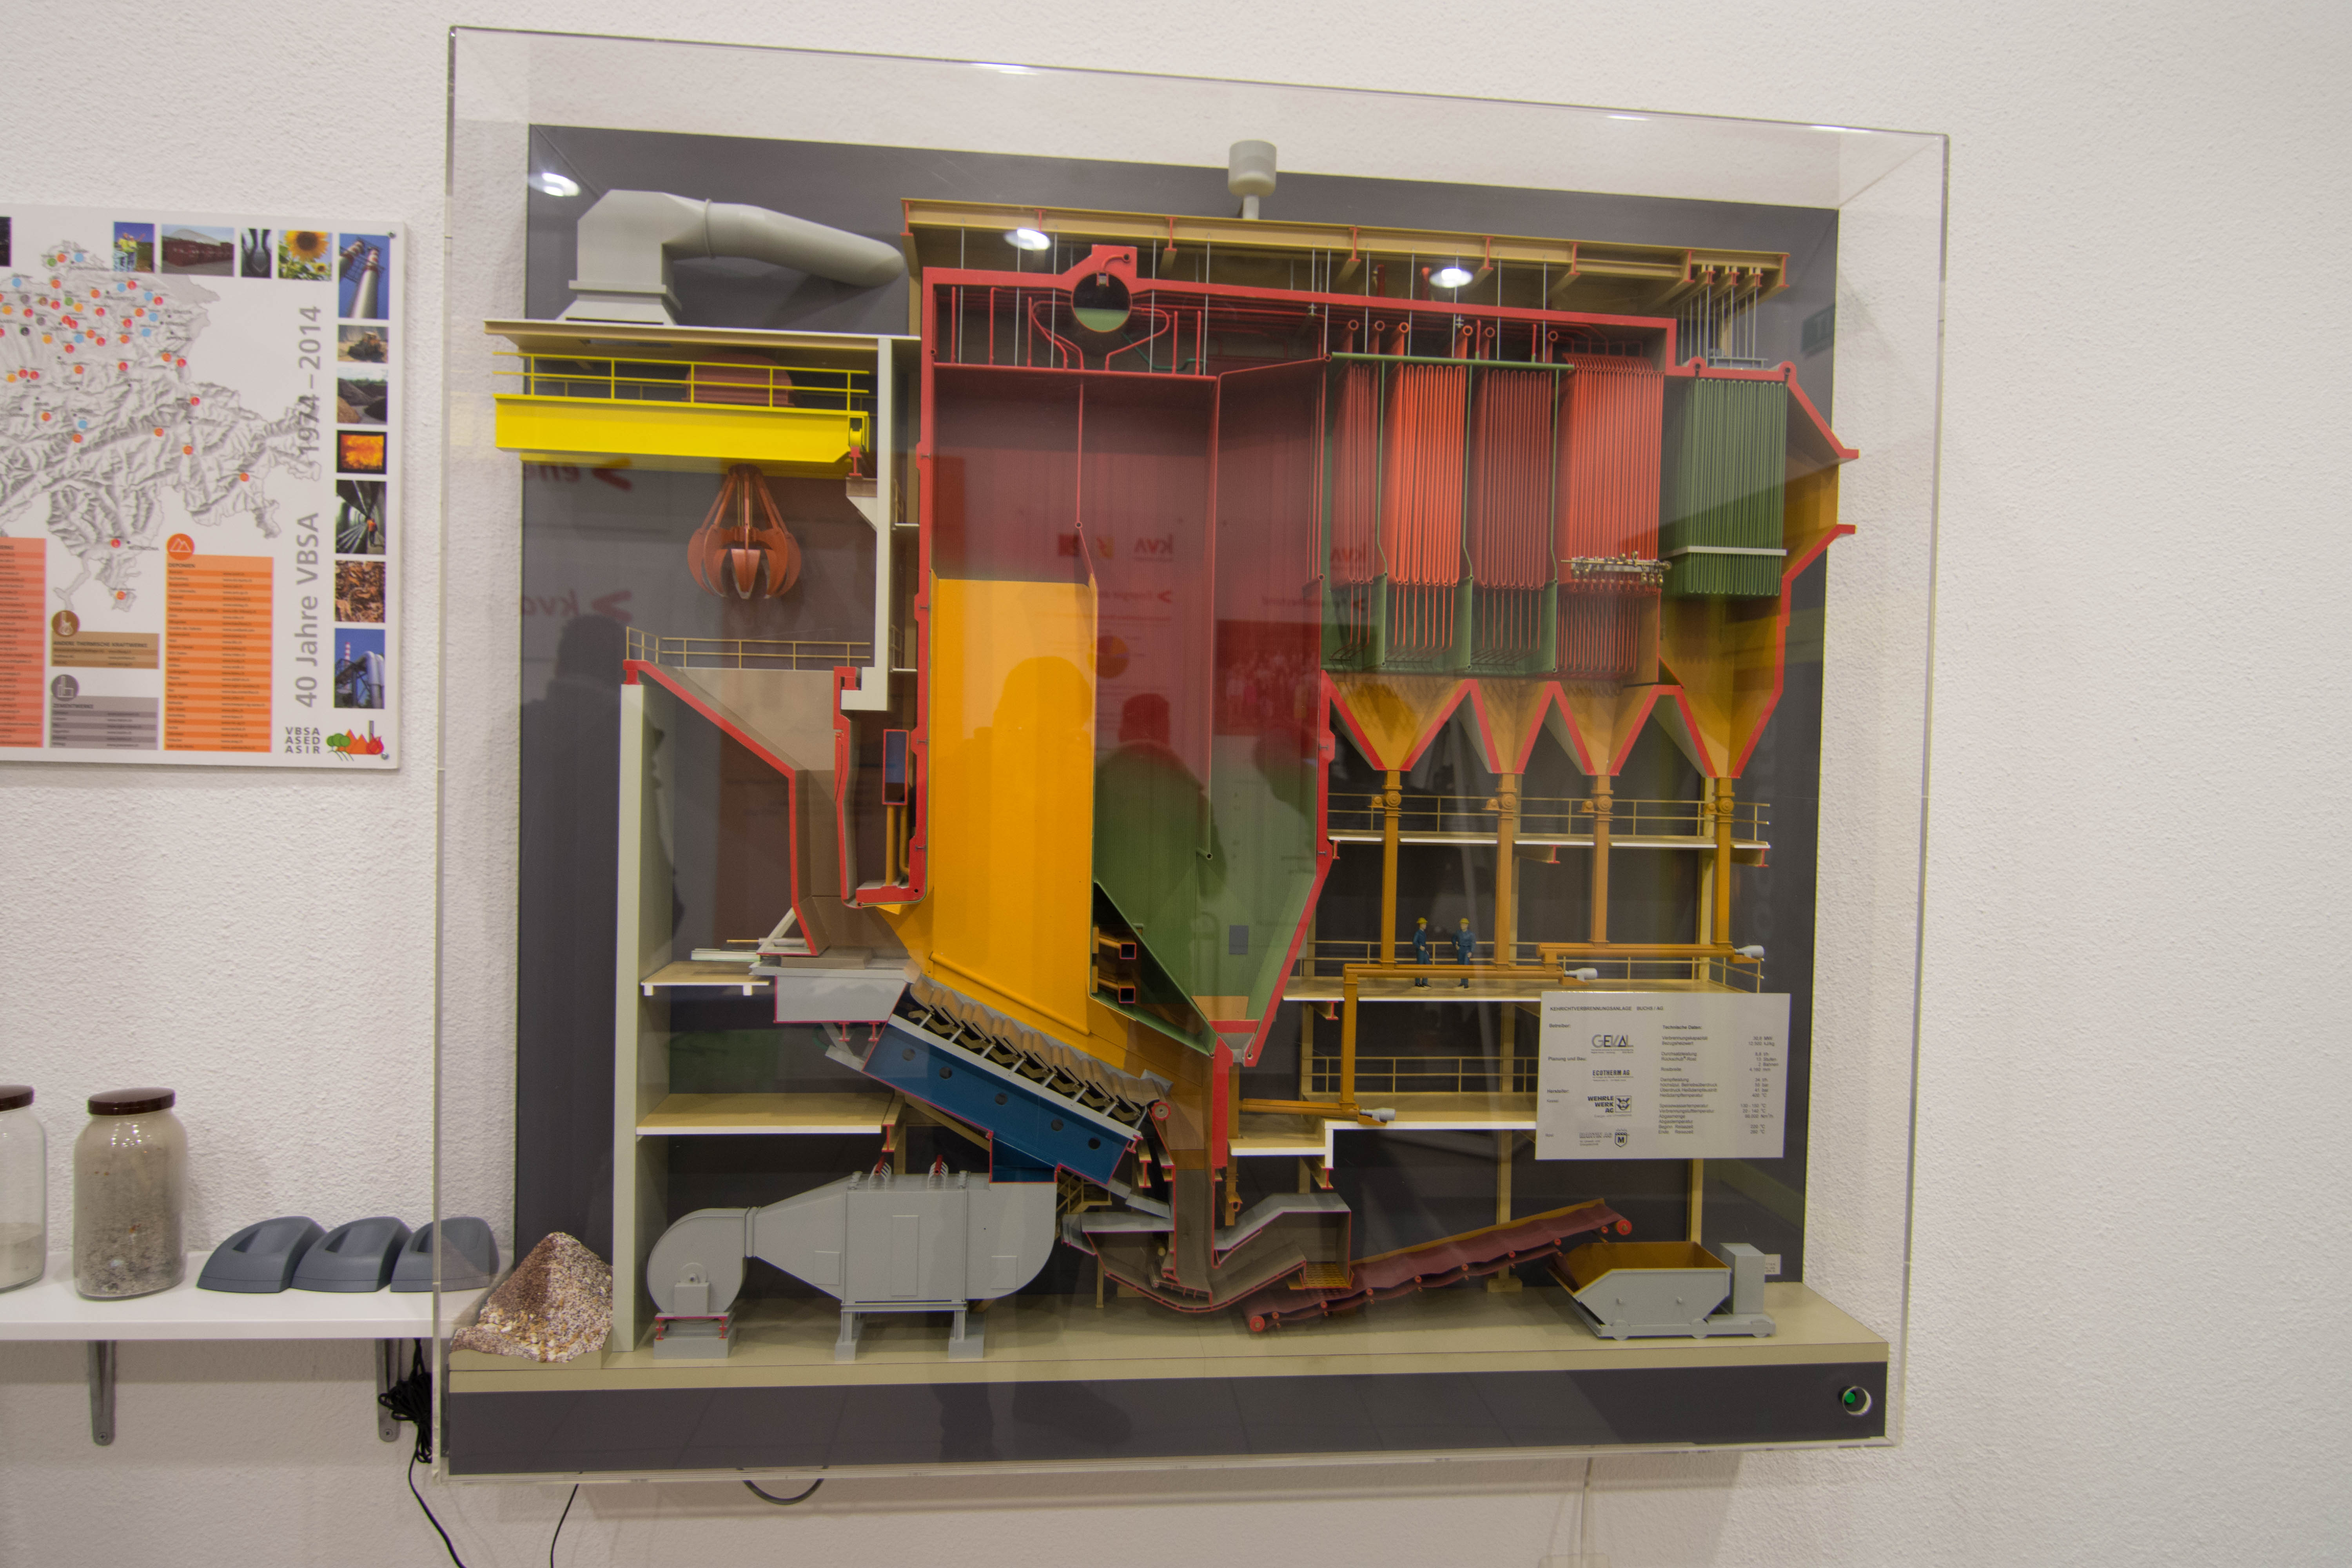
\includegraphics[width=10cm]{bilder/02_model.jpg}}
\end{center}

Viel interessanter als das Model, fand ich jedoch zwei Gläser, welche
direkt daneben standen. Das eine enthielt Schlacke, also Reste der
Verbrennung. Das zweite enthielt Staub welcher aus dem Rauch gefiltert
wurde. Von diesem Staub werden bis zu 35 kg pro verbrannte Tonne Abfall
herausgefiltert. Einerseits sehr beeindruckend, anderseits man sich
schon Gedanken darüber ob man die Reste die sie nicht heraus filtern
können wirklich in der Luft haben möchte.

\begin{center}
\frame{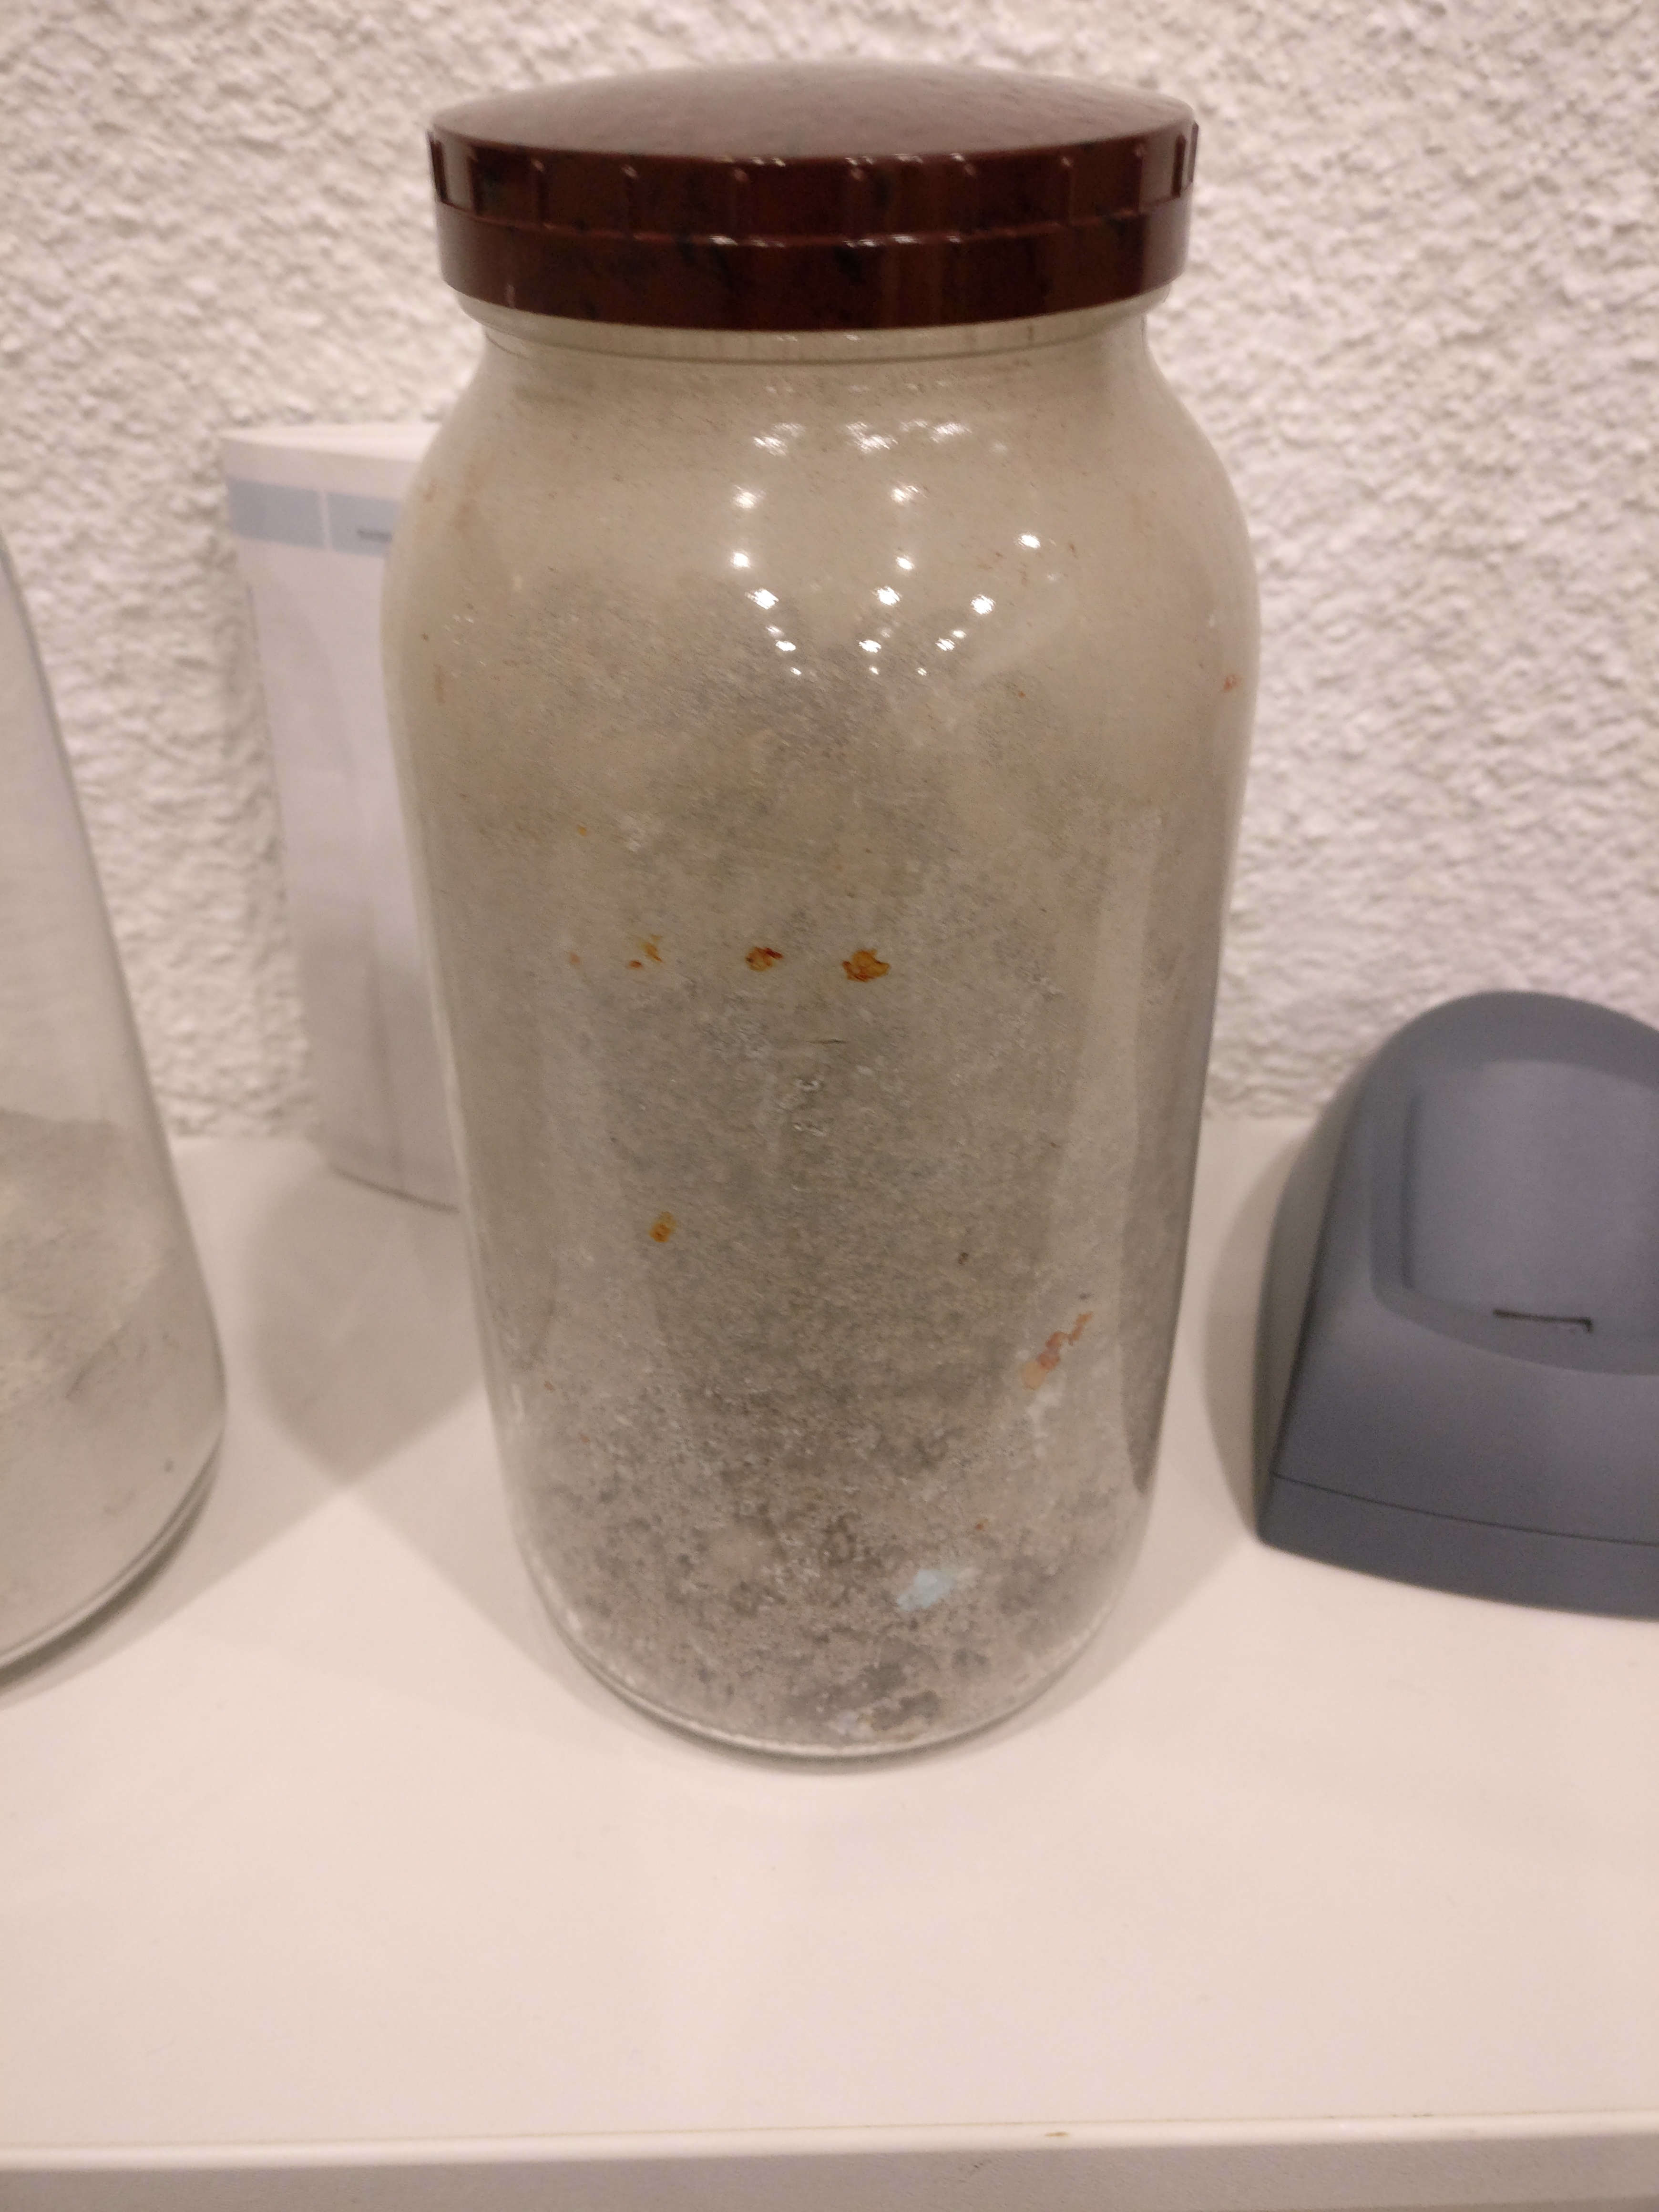
\includegraphics[scale=0.03]{bilder/03_schlacke.jpg}}
\frame{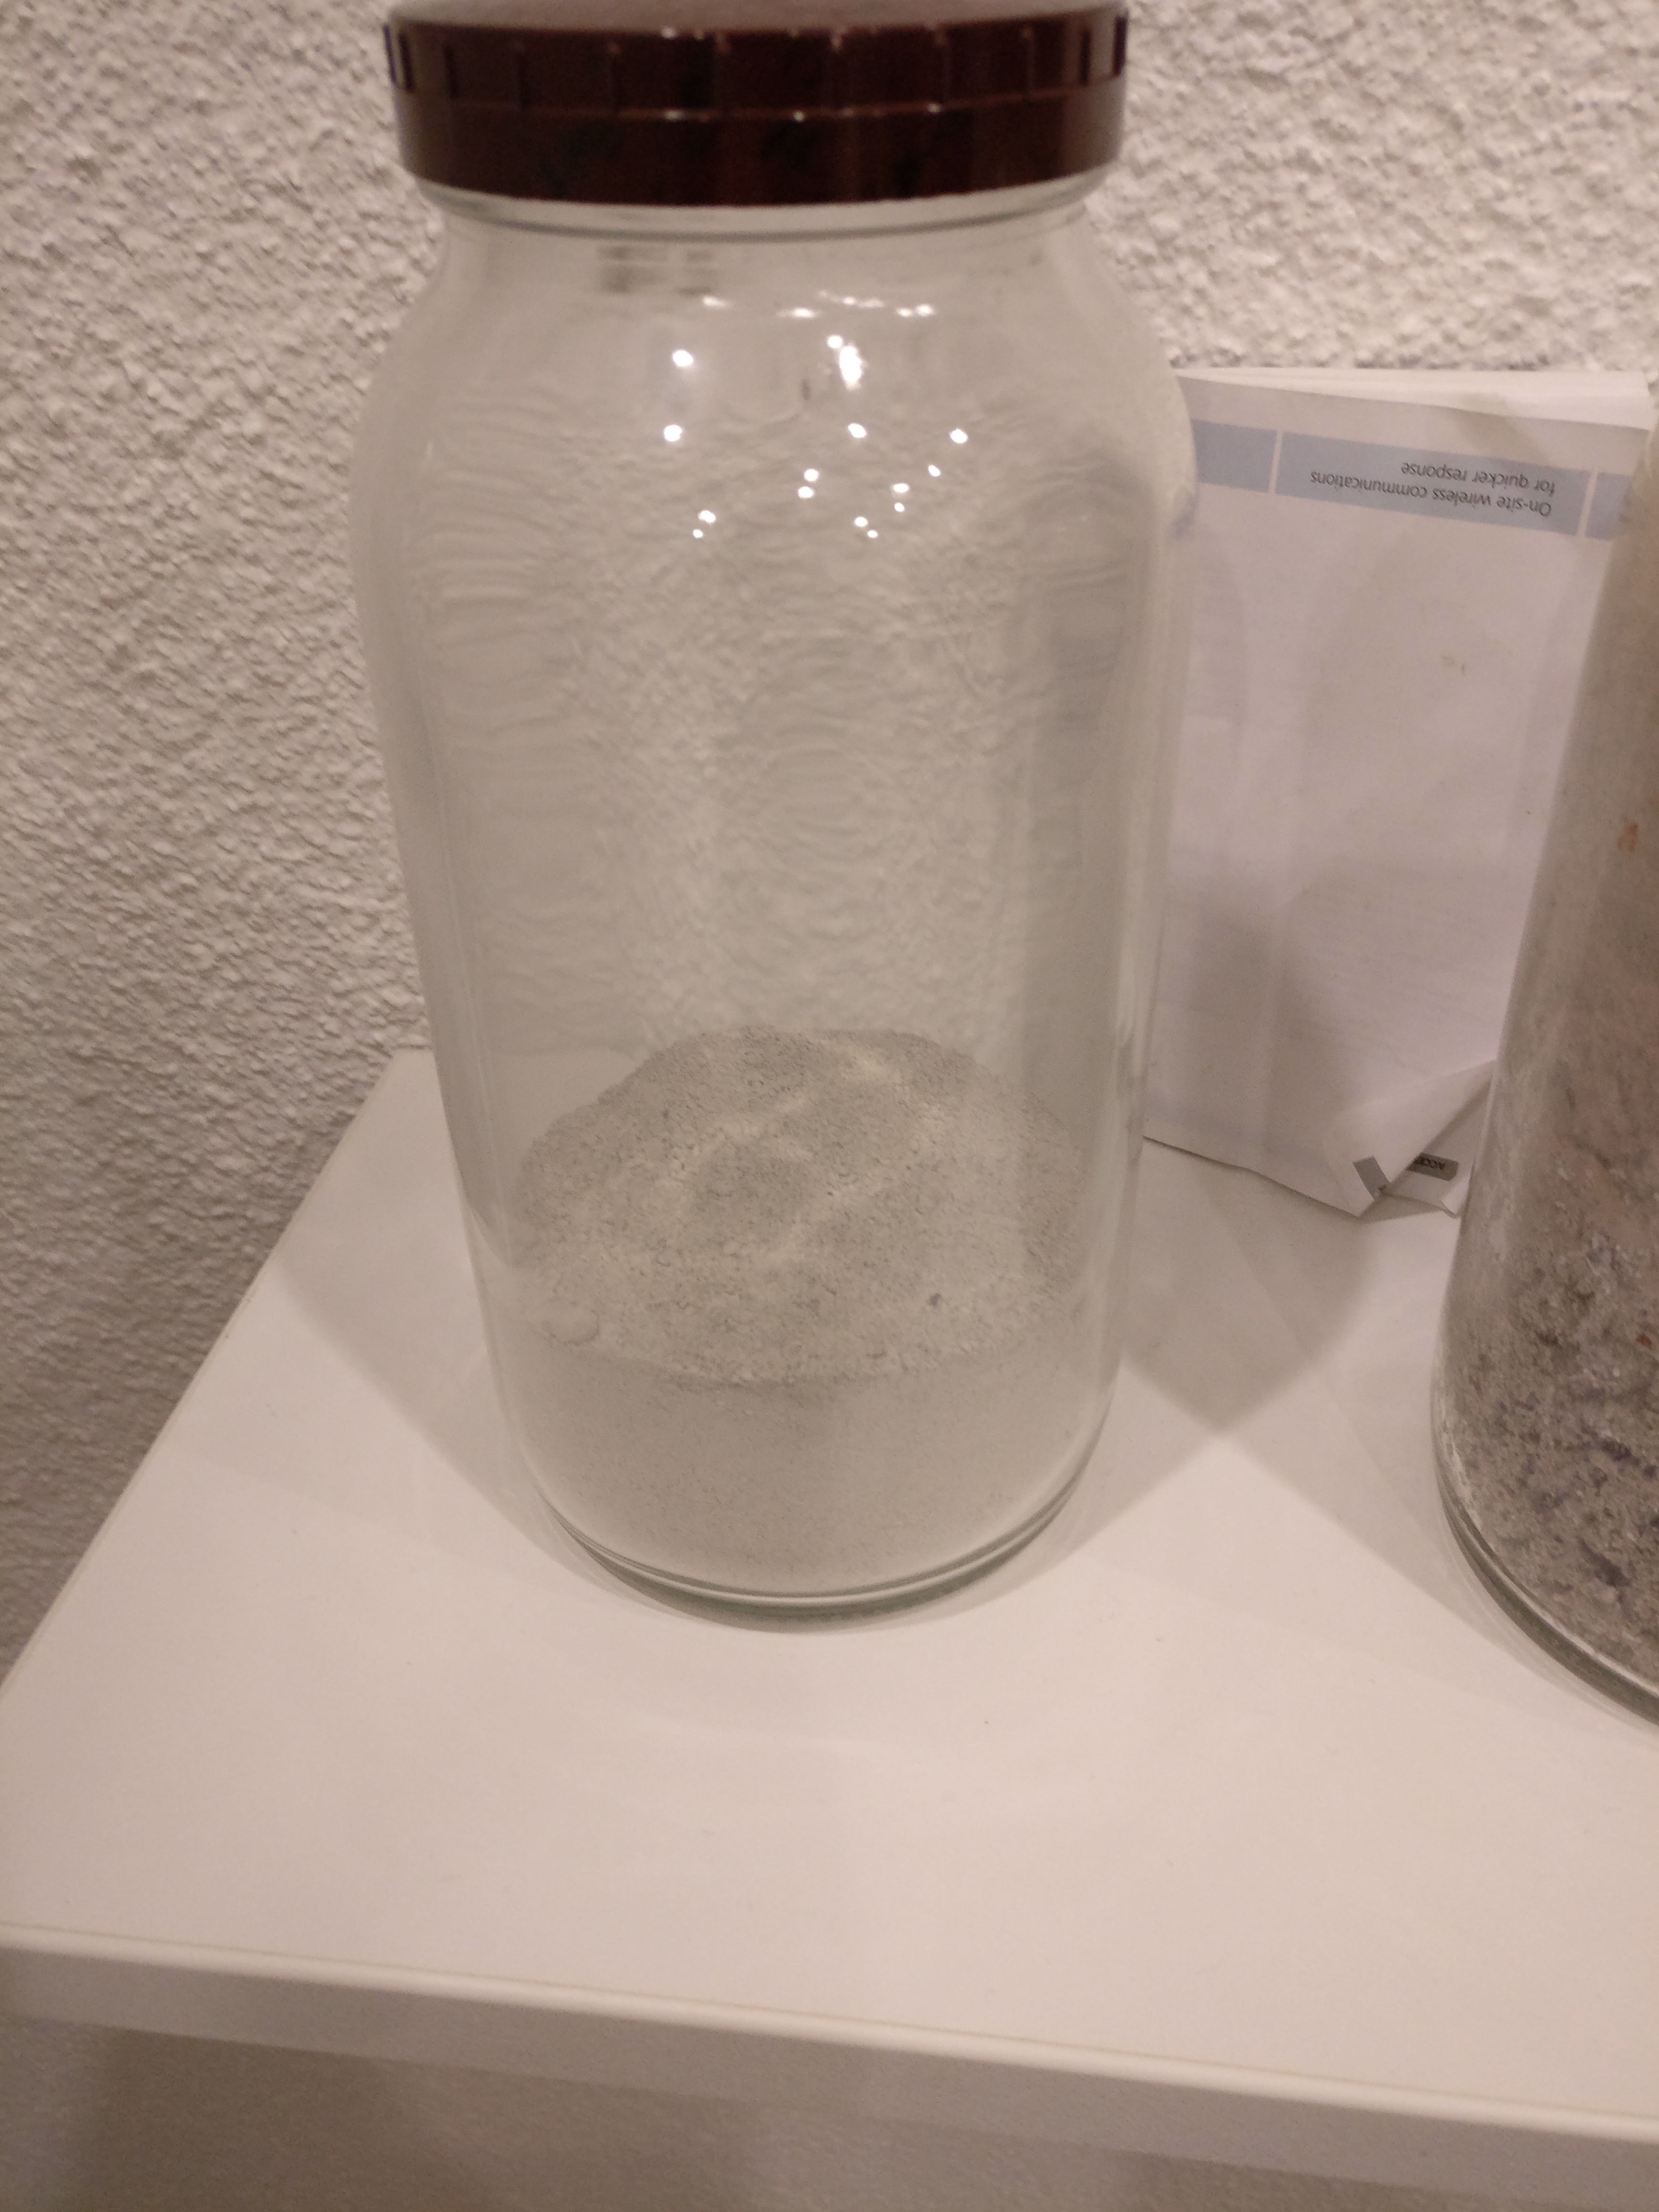
\includegraphics[scale=0.03]{bilder/04_staub.jpg}}
\end{center}

Hinzu kommt noch das der herausgefilterte Staub nach Deutschland
gebracht wird und dort in einem Salzbergwerk gelagert wird.
Dies wird allerdings nur noch bis 2021 möglich sein. Ab dann ist
diese Praxis verboten und der Staub muss auch gewaschen werden.

\subsection{17:55 Uhr}
\label{sec-2-5}
Nach der Erklärung der Anlage zeigte und Frau Fürsinger noch eine
Auswahl an skurriler Gegenstände welche die Mitarbeiter der Anlage in
der Schlacke gefunden hatten. Solche Gegenstände findet man weil der
Abfall ``nur'' mit 800 - 1000\(^{\circ}\)C. Metall sowie Glas benötigen
jedoch wesentlich höhere Temperaturen um zu brennen. Aus
diesem Grund gibt es für diese Materialien auch separate
Sammelstellen.  

\begin{center}
\frame{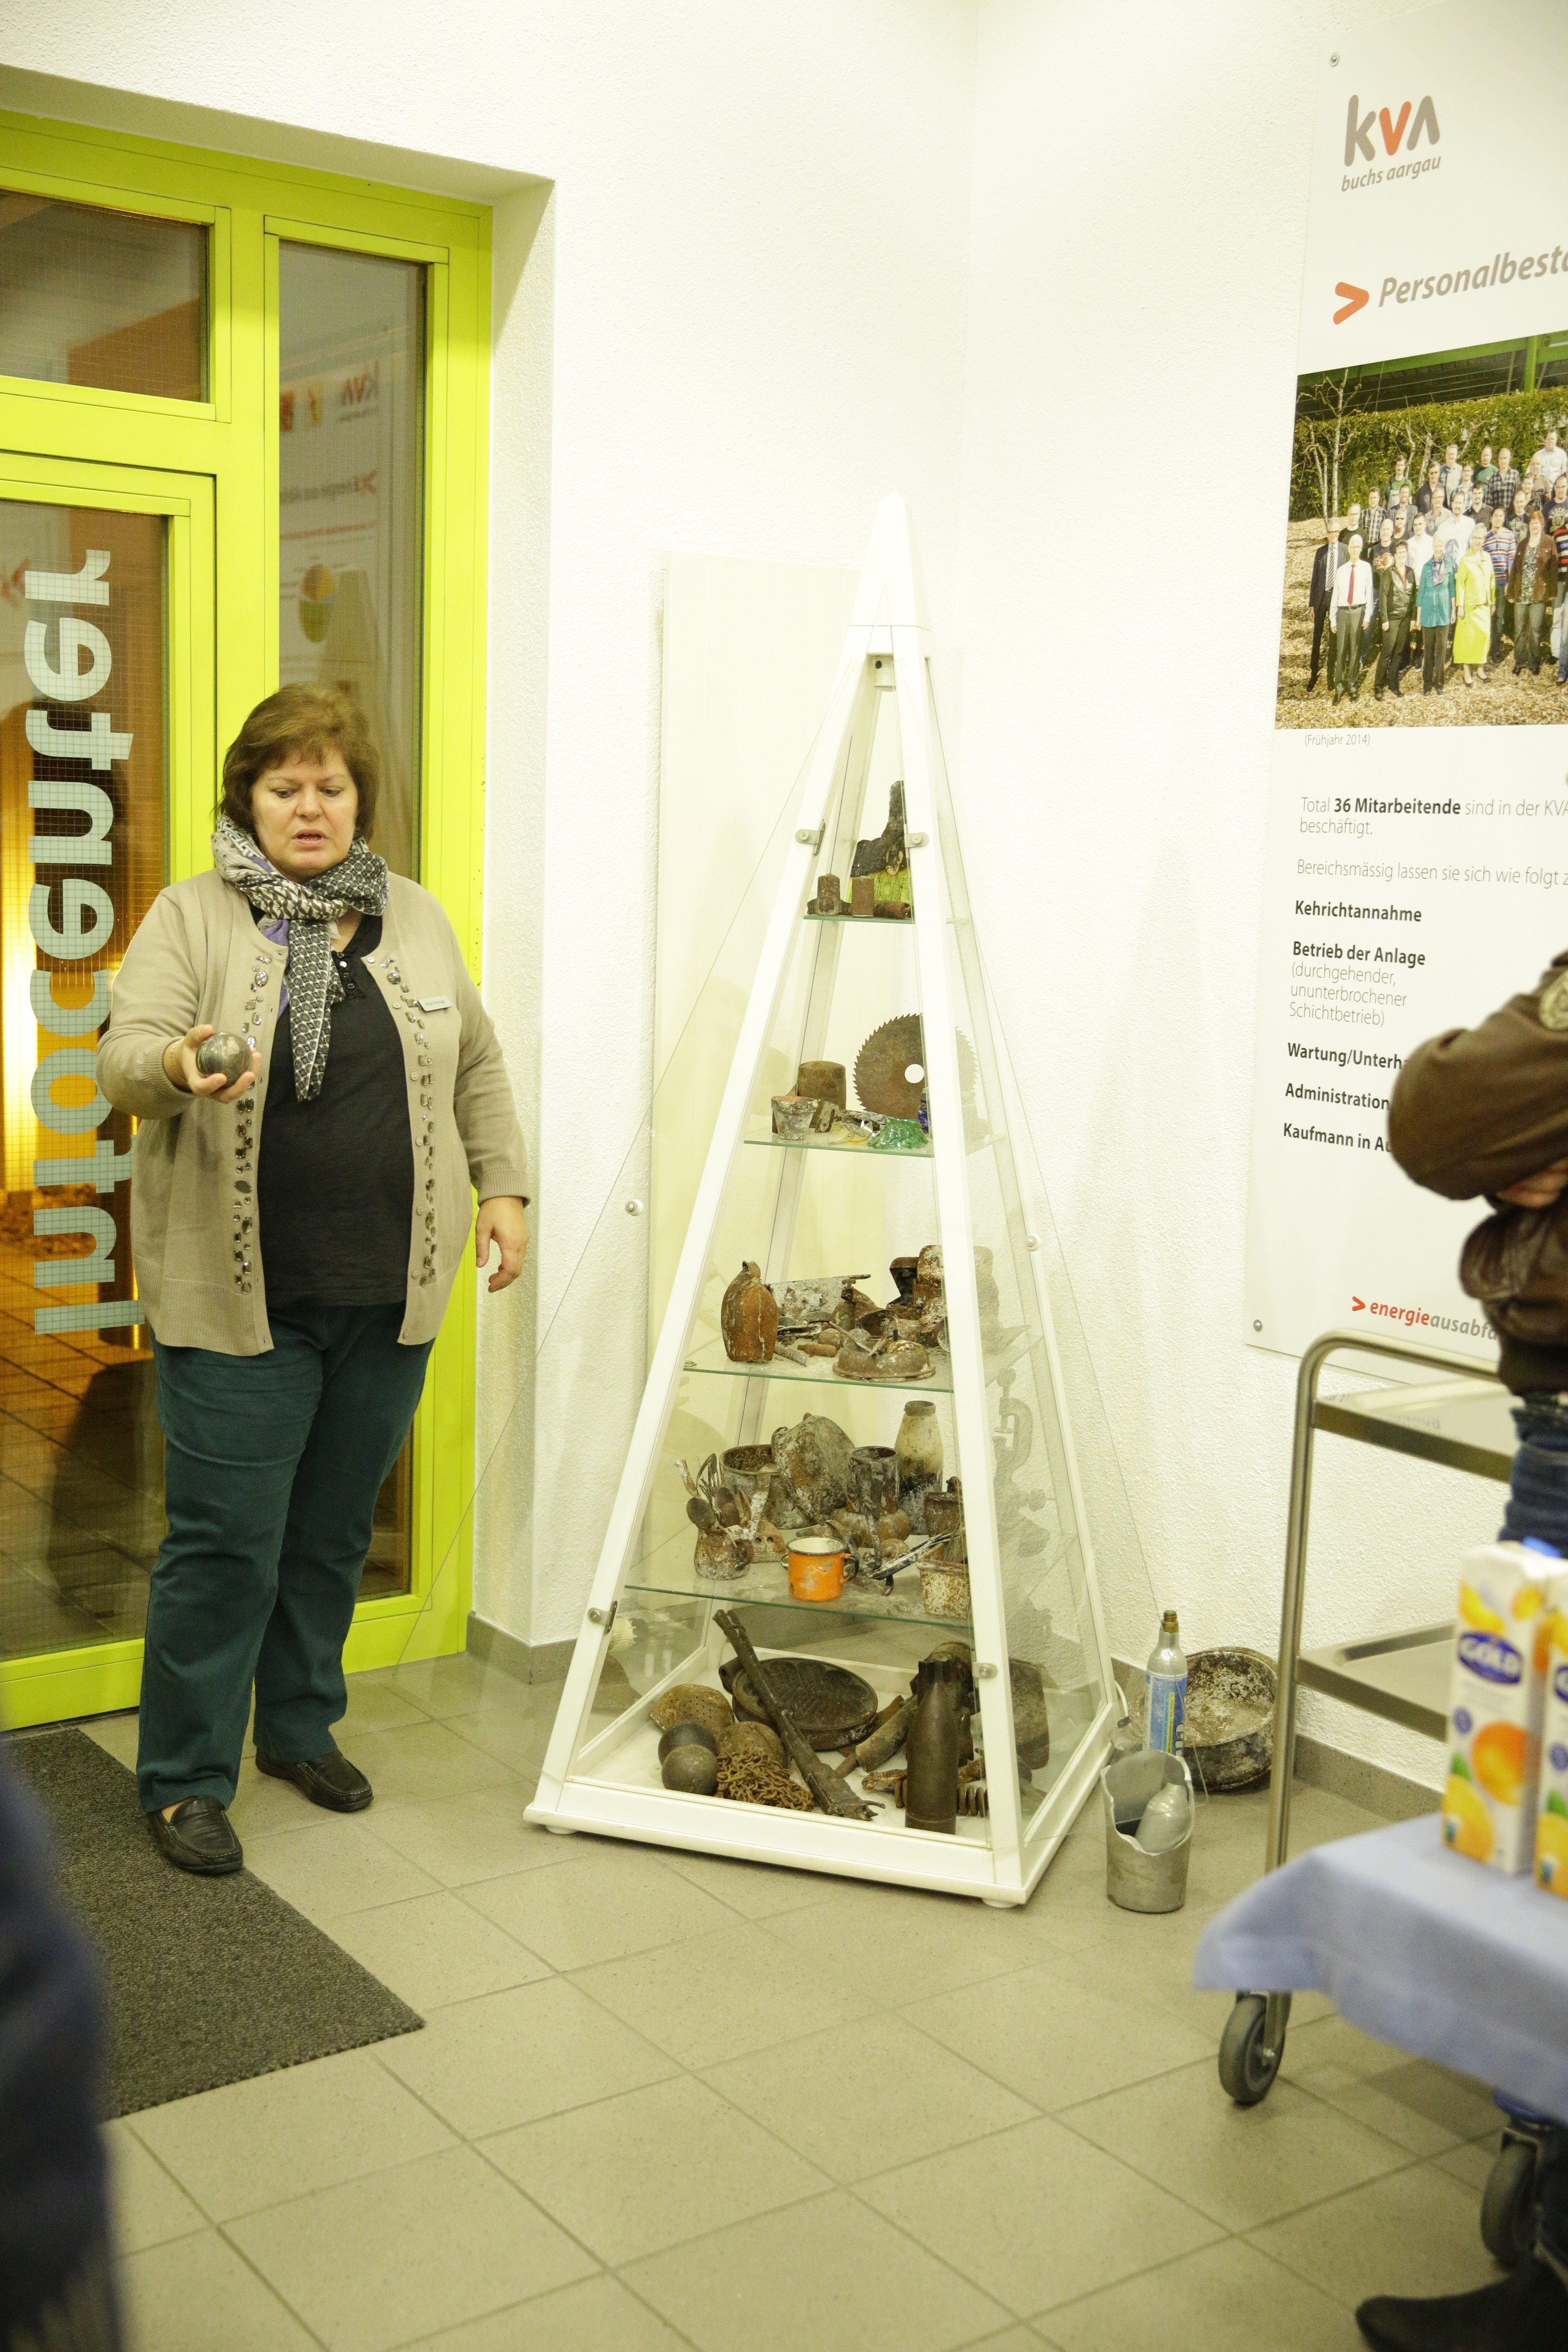
\includegraphics[scale=0.04]{bilder/05_gegenstaende.jpg}}
\end{center}

Nichtsdestotrotz werfen die Leute alles mögliche fort. Die Funde
reichen von gewöhnlichen Besteck bis zu Geschossen. Etwas schmunzeln
musste ich als Frau Fürsinger uns voller Stolz ihren neuesten Fund
präsentierte, eine Lochzange.

\subsection{18:10 Uhr}
\label{sec-2-6}
Anschliessend fuhren wir mit dem Lift ein paar Etagen höher um die
Kräne zu besichtigen welche den Müll im Bunker durchmischen und auf
den Förder geben.  Mit dem Förderer wird der Müll dann Richtung und
durch den Ofen transportiert. 

\begin{center}
\frame{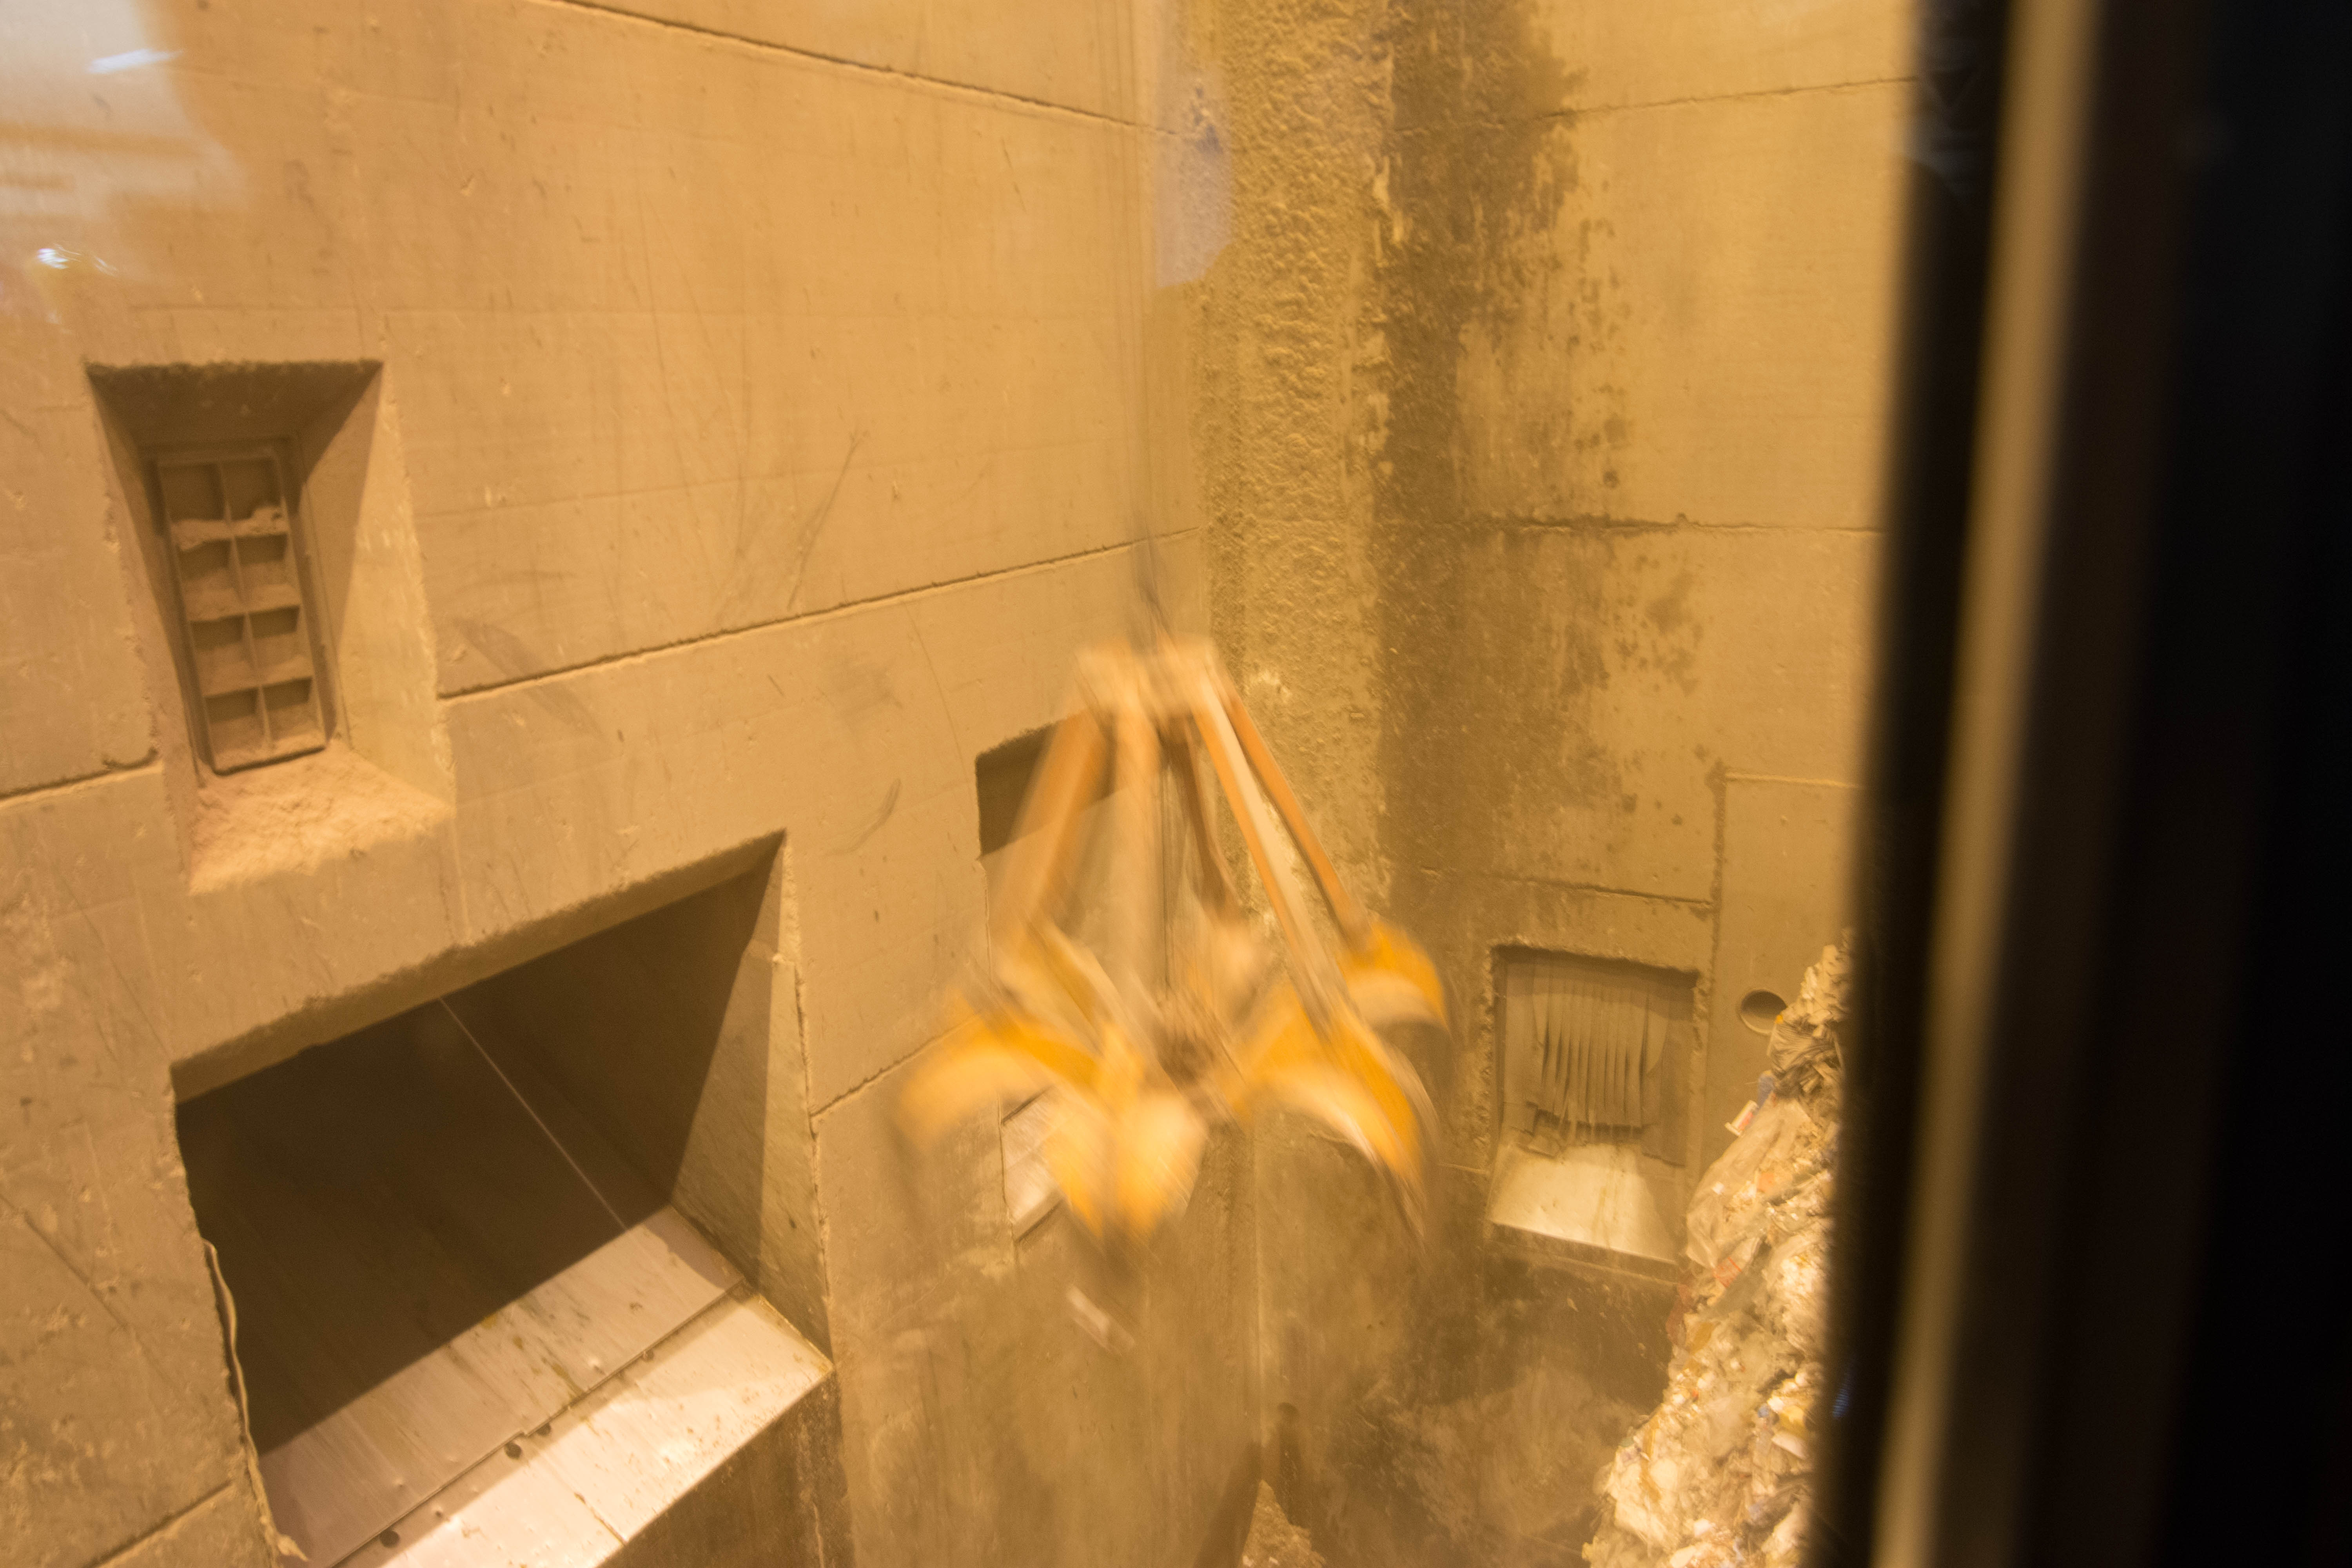
\includegraphics[scale=0.019]{bilder/06_kran.jpg}}
\frame{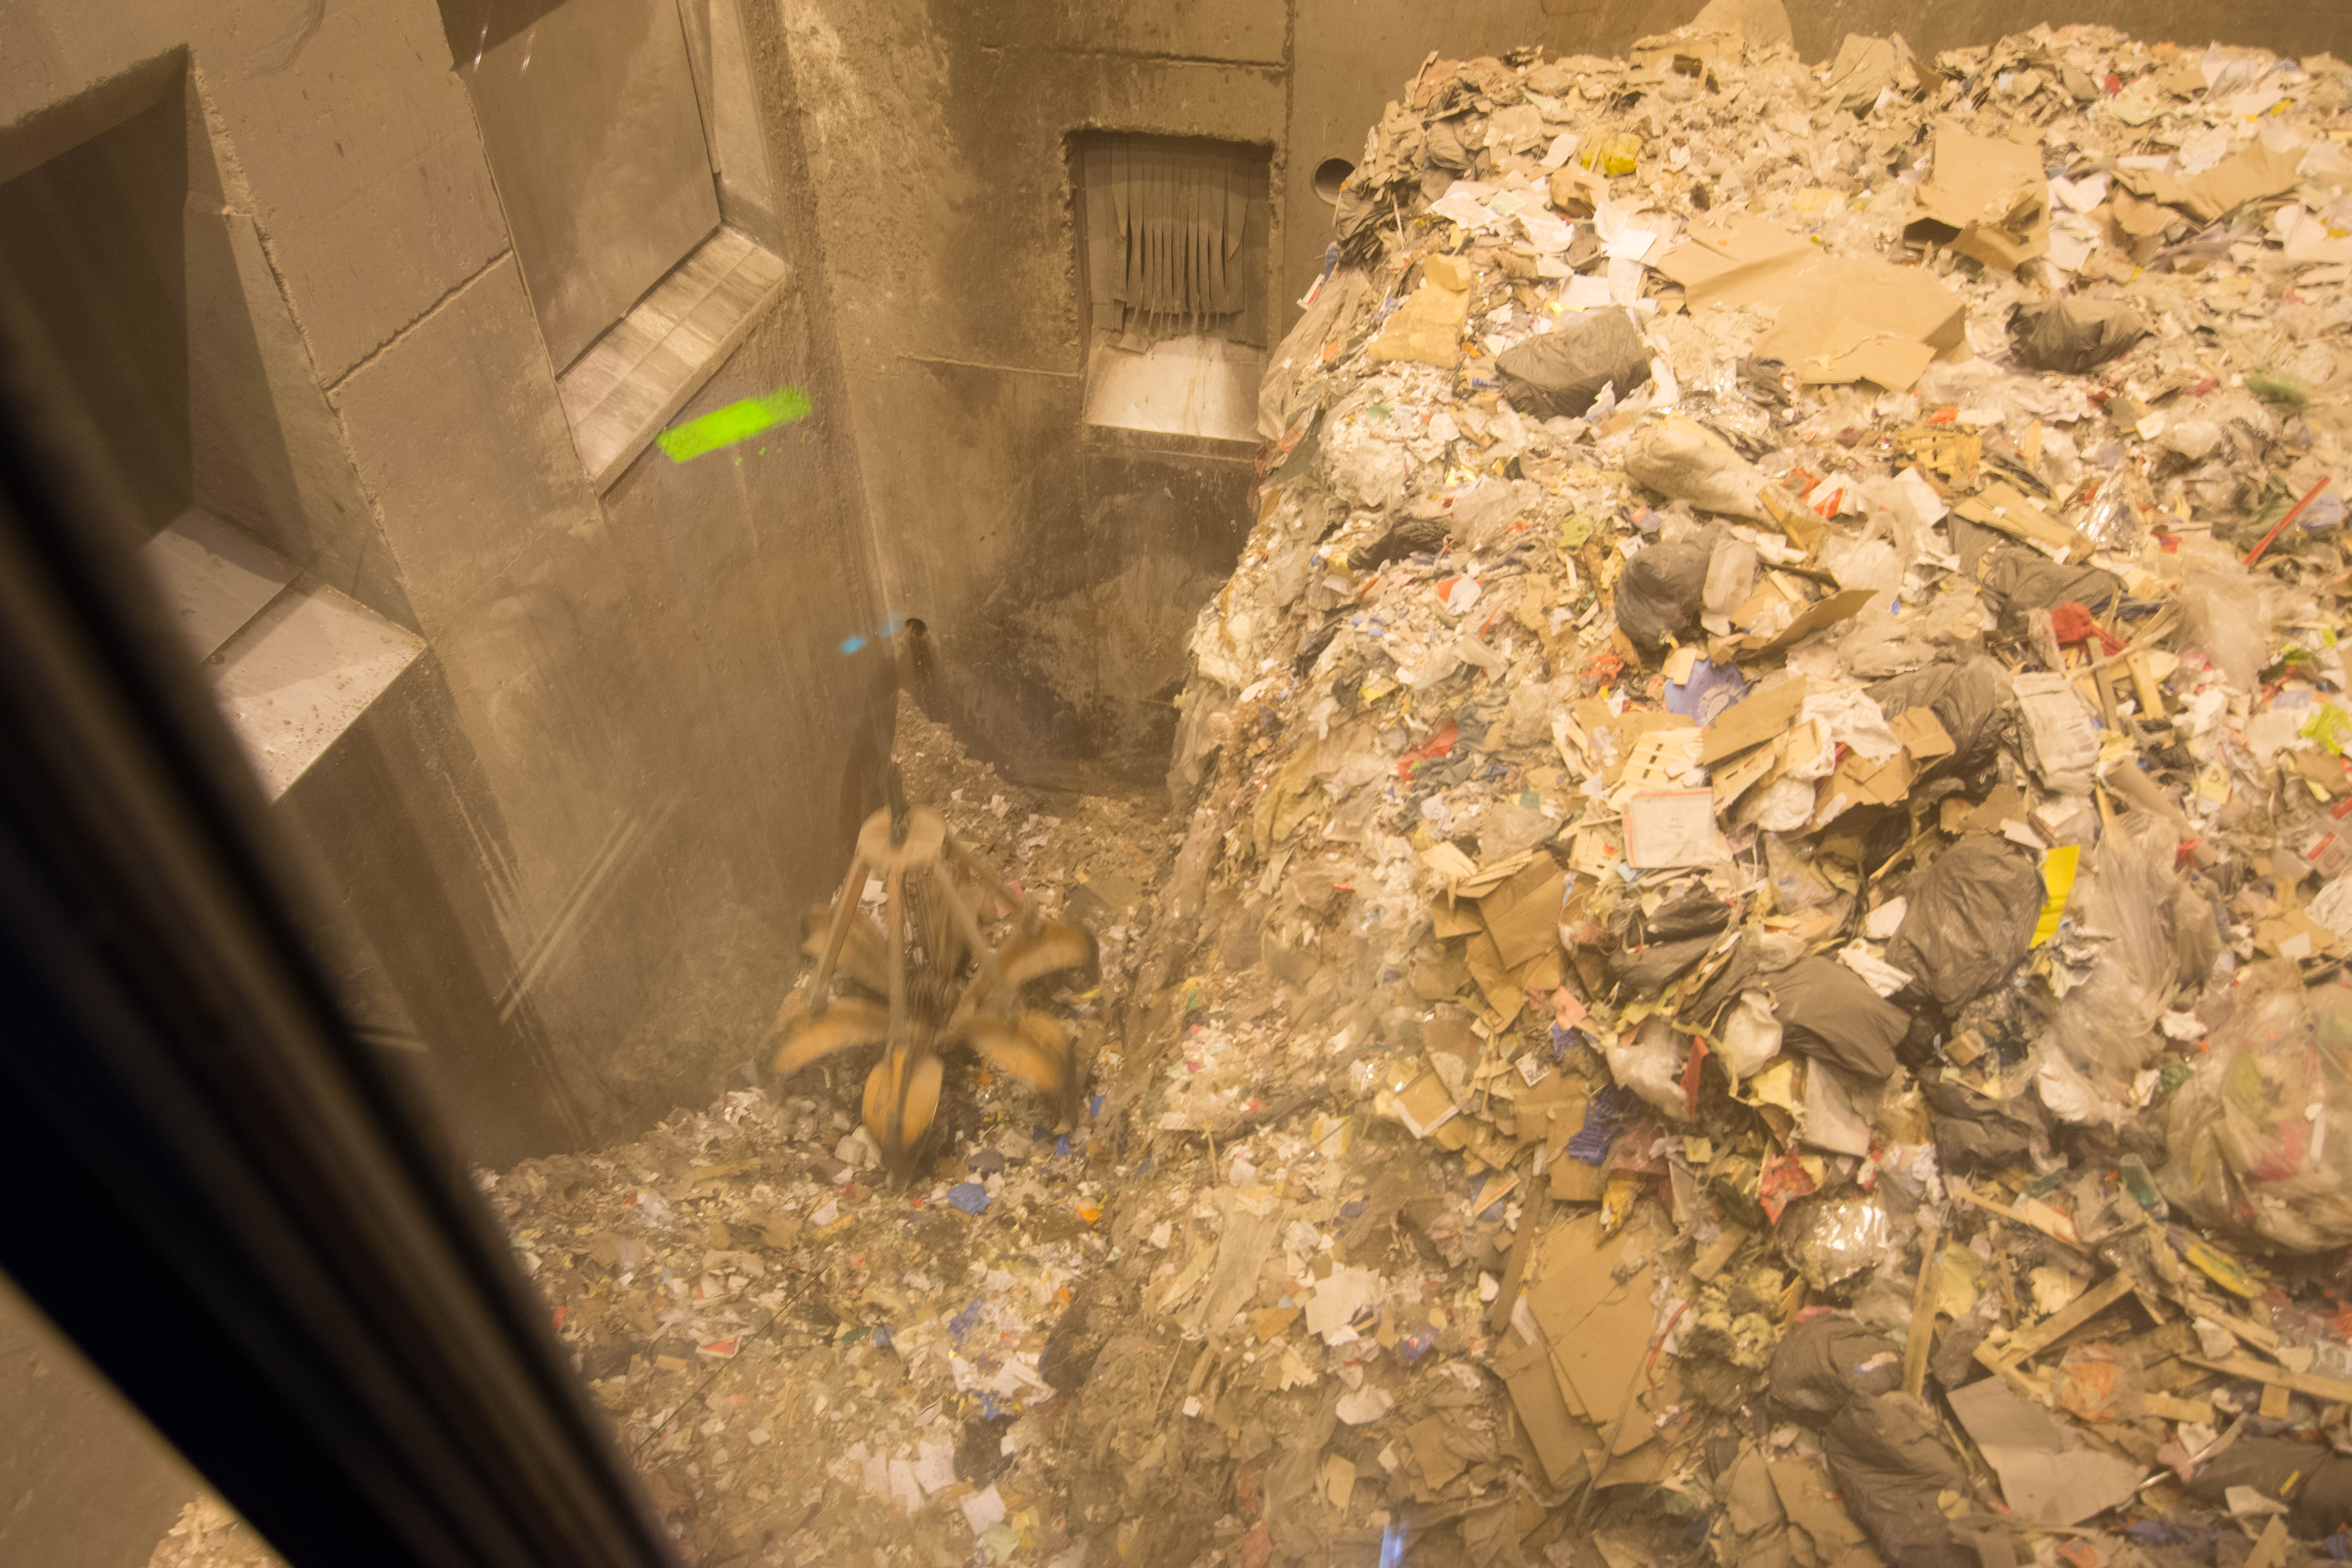
\includegraphics[scale=0.019]{bilder/07_kran.jpg}}
\frame{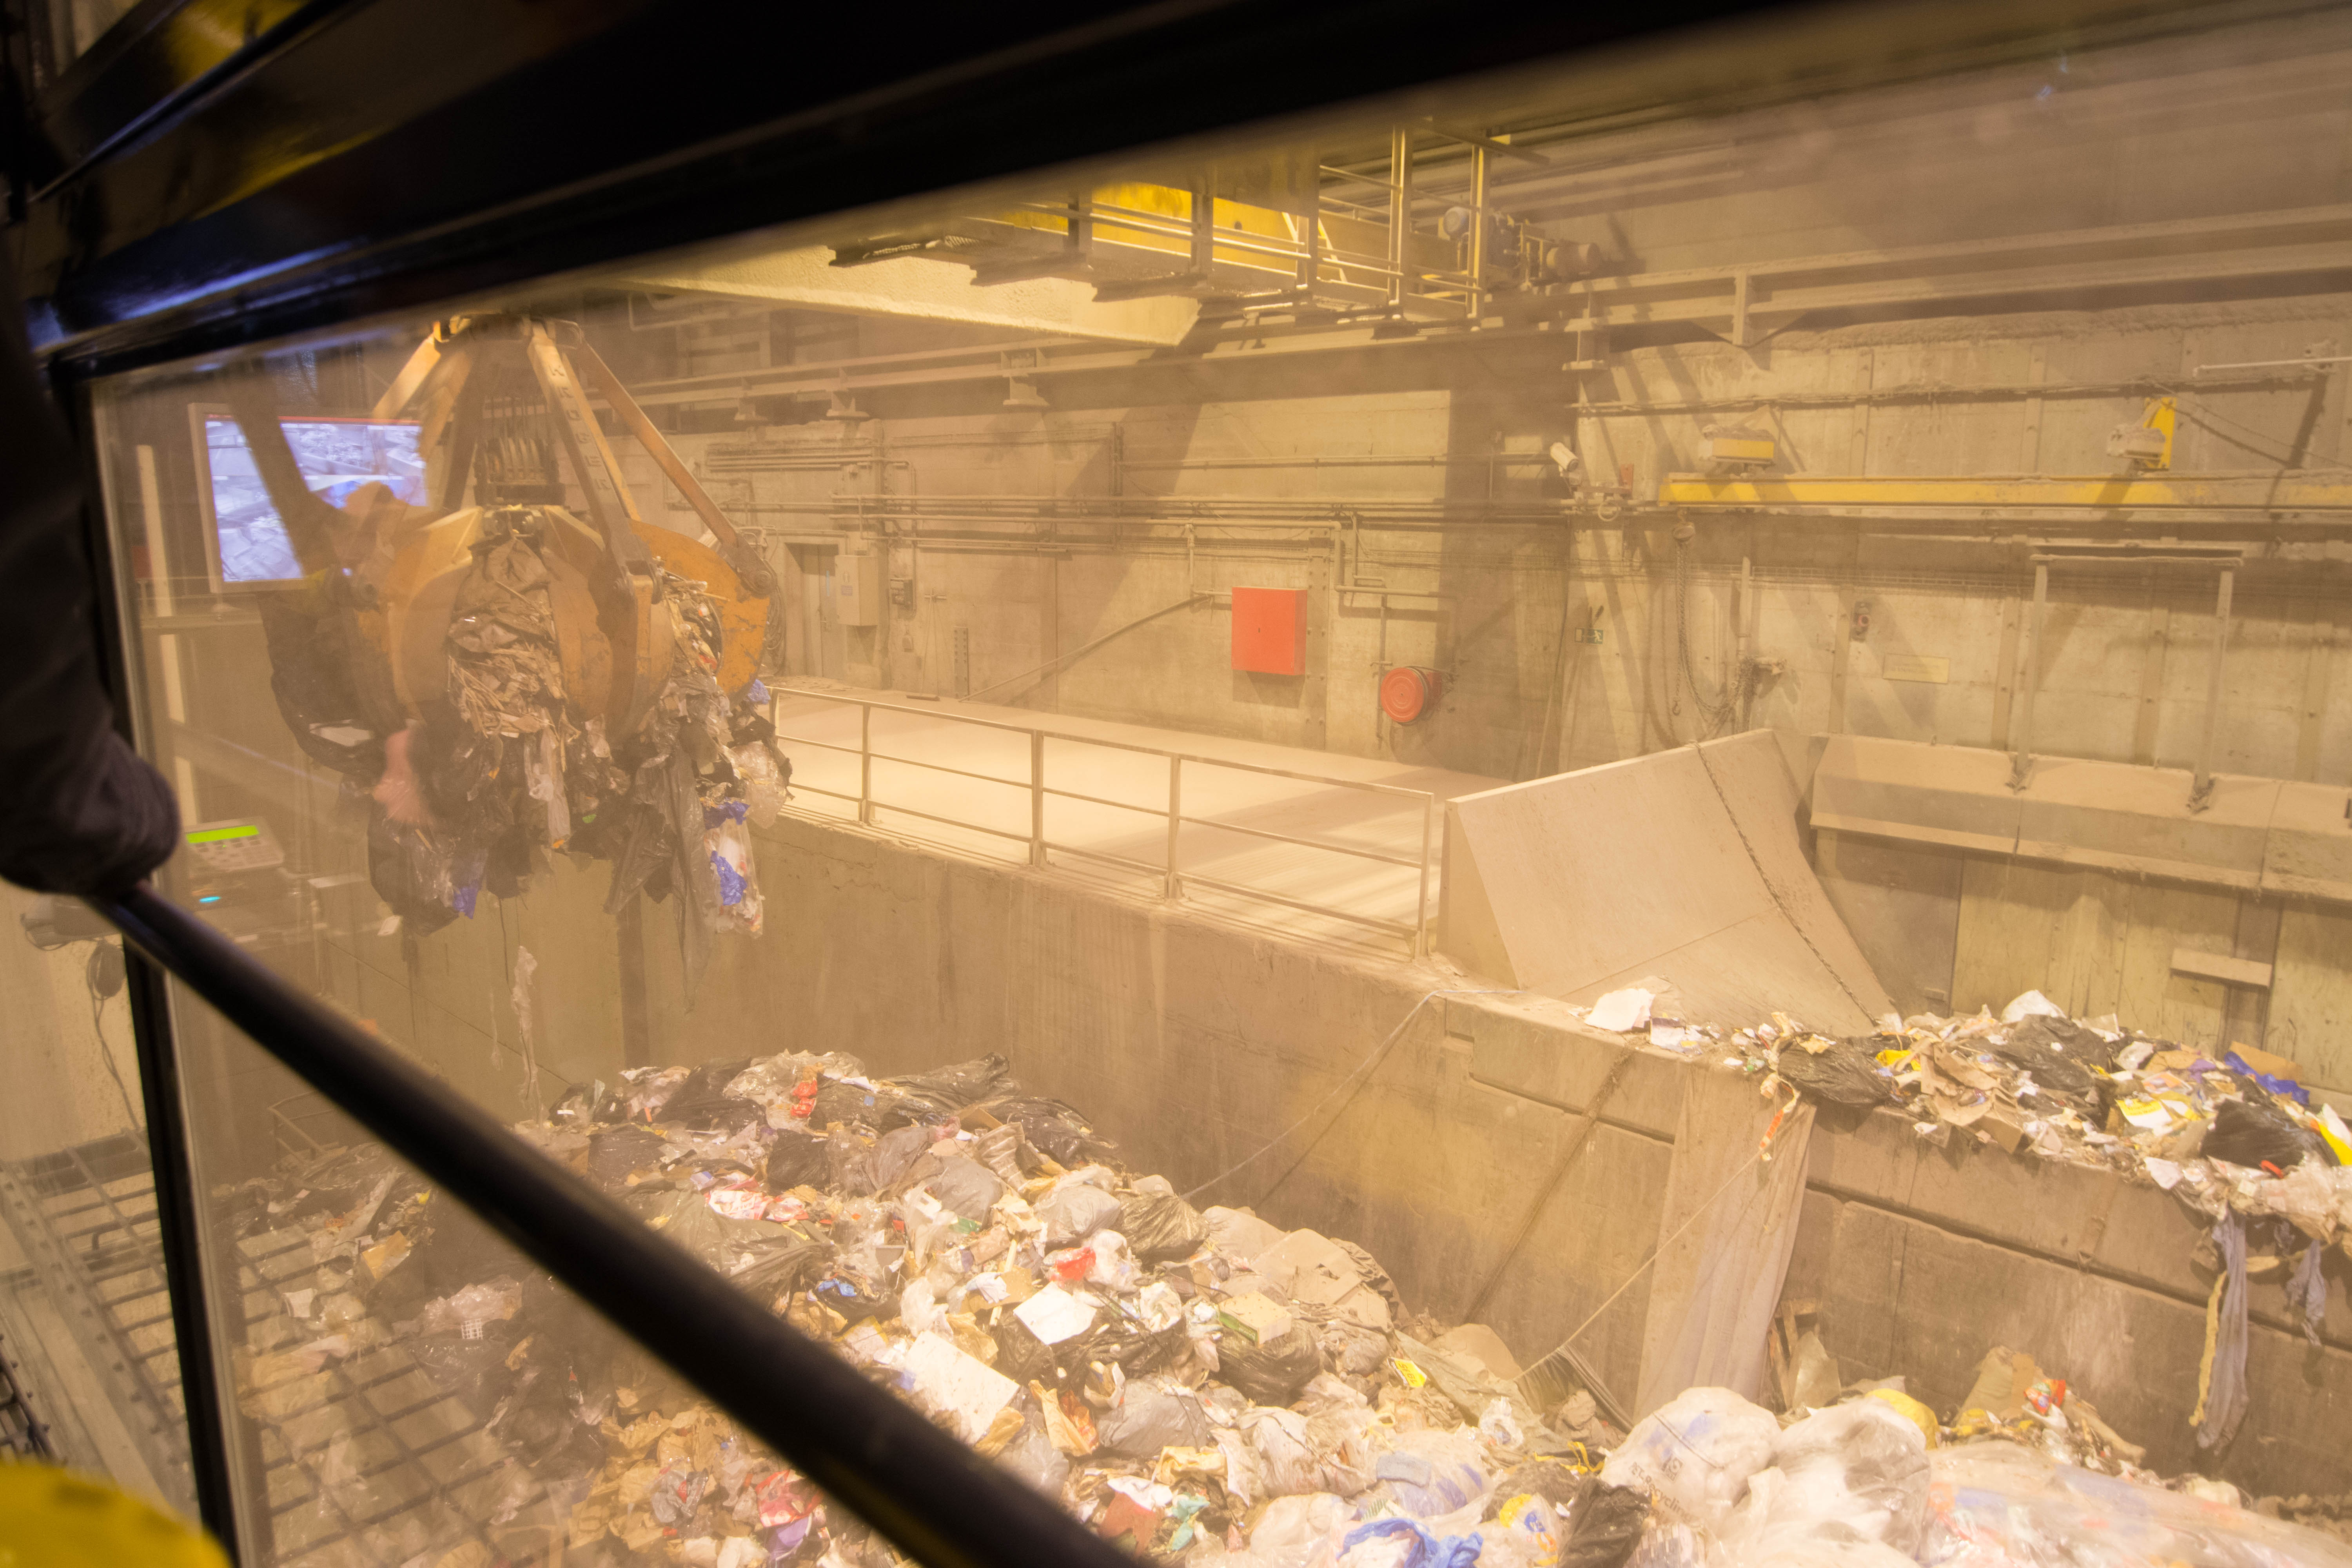
\includegraphics[scale=0.019]{bilder/08_kran.jpg}}
\end{center}

Ich finde es ist immer wieder erstaunlich zu sehen mit welcher
scheinbaren Leichtigkeit solche grosse Maschinen, sich und ihre Lasten
bewegen.  

Das Durchmischen ist aus mehreren Gründen wichtig. Einerseits ist der
Müll oft feucht, wenn er bei der KVA ankommt. Durch das Durchmischen
wird er getrocknet, wodurch er besser brennt. Desweiteren kann es durch
den feuchten Müll zu sogenannten Bunkerbränden kommen, wenn er zu fest
zu gären beginnt. Zu guter Letzt ist es natürlich auch schlicht und
einfach wichtig das man die ganze Sache etwas umschichtet. Ansonsten
hat man schnell ein Platzproblem.

\subsection{18:20 Uhr}
\label{sec-2-7}
Nach den Kränen ging es weiter zu den Öfen. Diese befanden sich in
einer hohen Halle. Insgesamt würde die KVA Platz für 3 Öfen bieten
wobei zur Zeit nur zwei installiert sind. Das Feuer in den
Verbrennungsanlagen war überraschend hell.

\begin{center}
\frame{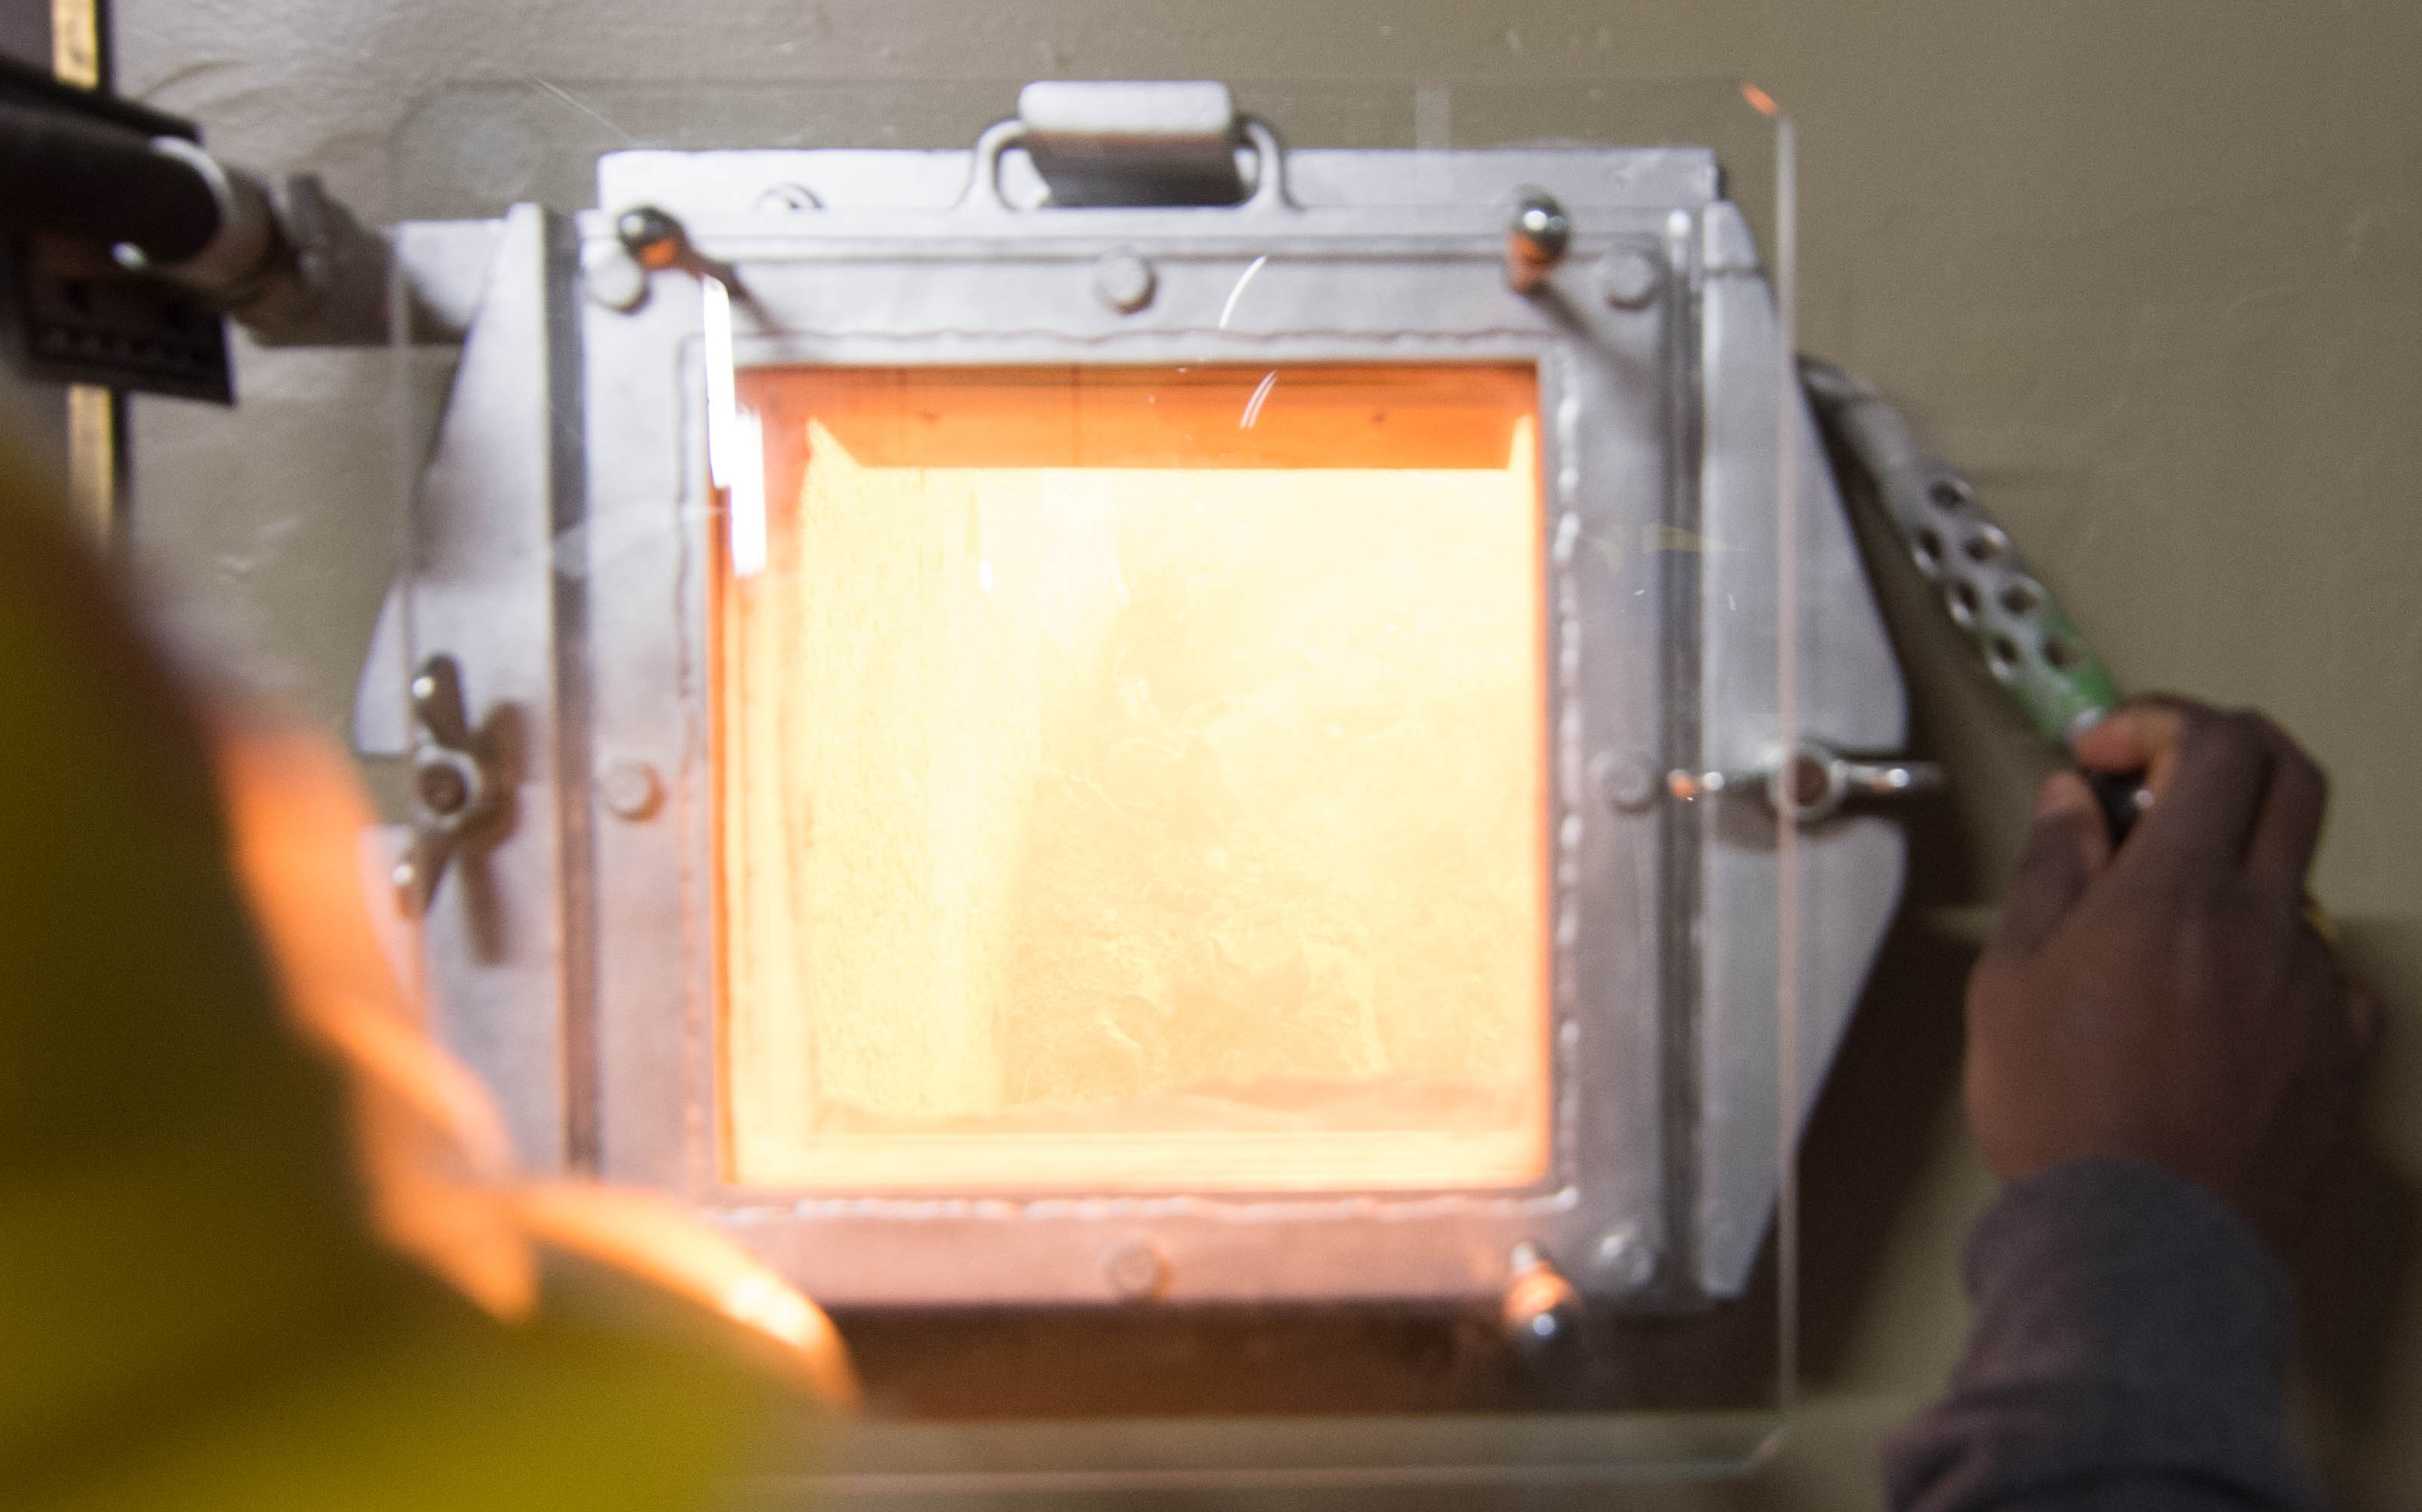
\includegraphics[width=10cm]{bilder/09_ofen.jpg}}
\end{center}

Die Öfen in Gang zu bringen wenn sie erloschen sind ist eine
erstaunlich simple Sache. Wenn wieder genügend Material im Ofen ist,
wirft man einfach einen mit Petrol durchtränkten Lumpen in den Ofen
und das Feuer beginnt wieder zu brennen wobei eine gute Luftzufuhr
dafür sorgt, dass das Feuer nicht erstickt. Nach dem Abschalten dauert
es ca. einen Tag bis man die Öfen betreten kann. So wirklich angenehm
kühl sind sie dann aber noch lange nicht.

\subsection{18:30 Uhr}
\label{sec-2-8}
Im Anschluss zu den Öfen begaben wir uns zum Turbinenraum. Dieser war
relativ unspektakulär. Trotzdem ist er von essenzieller Wichtigkeit da
hier der gesamte Strom der KVA produziert wird. Zu meinen grossen
erstaunen war es in diesem Raum wärmer als im Ofenraum. Aber Reibung
erzeugt ja bekanntlich auch Wärme.

\subsection{18:35 Uhr}
\label{sec-2-9}
Auch wärend der Führung gab der Turbinenraum nicht allzuviel her
weshalb wir nach 5 Minuten bereits zum Kontrollraum weitergingen.  Der
Kontrollraum war ein länglicher, relativ unspektakulärer Raum. In der
Mitte befand sich ein langer Tisch an welchem ungefähr 10 Monitore
montiert waren. Diese zeigten etwa Bilder von Überwachungskameras
welche den äusseren Bereich, sowie auch Skalen von analogen Sensoren
überwachten.  Zudem waren auf den Bildschirmen auch diverse
Computerprogramme zu sehen welche den Status der Anlage
anzeigten. Eine Meldung welche sich mit einem Alarmton bemerkbar
machte liess unsere Gruppe kurz aufschrecken. Es handelte sich bei der
Meldung jedoch um nichts Ernstes.

\begin{center}
\frame{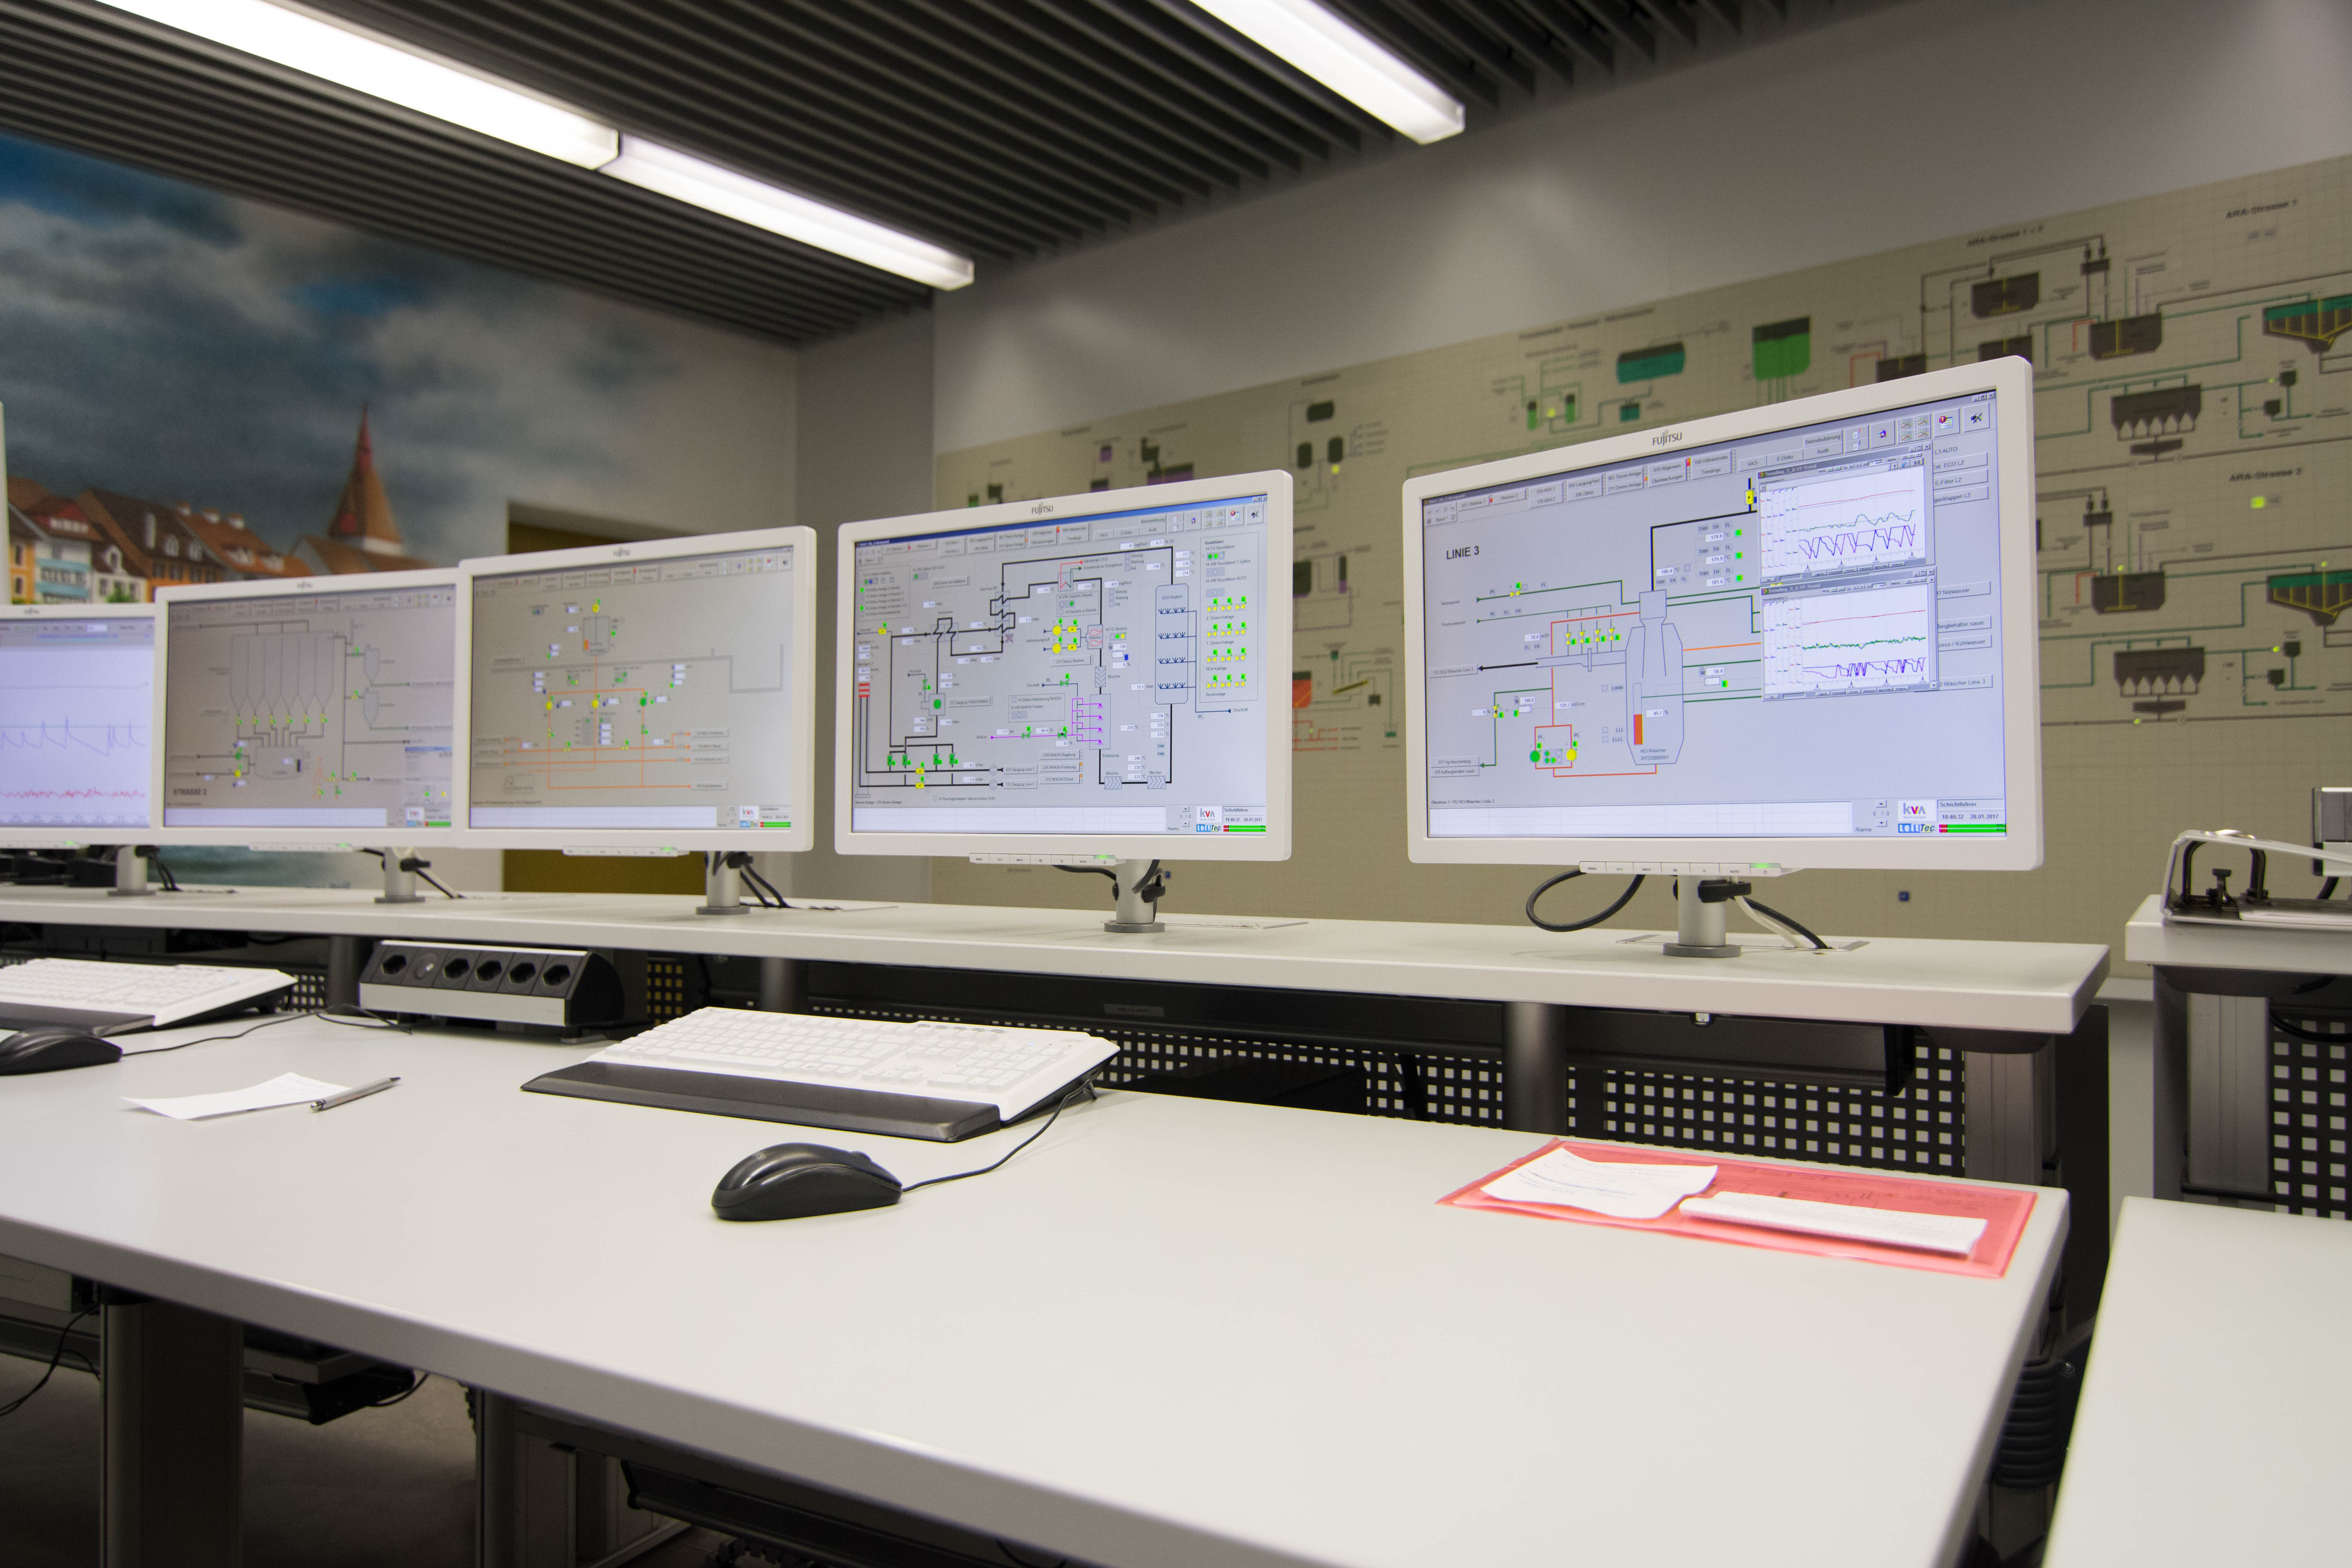
\includegraphics[width=10cm]{bilder/10_kontrolle.jpg}}
\end{center}

\subsection{18:45 Uhr}
\label{sec-2-10}
Durch den Raum mit dem Rauchgaswäscher ging es dann weiter in die
Abwassereinigung. Der Rauchgaswäscher wird benötigt damit die Abgase
der KVA von schädlichen Stoffen gereinigt werden können.  Dabei werden
etwa Salzsäure, Schwefeldioxid und Quecksilber aus dem Rauch
gefiltert. Im letzten Schritt wird dann noch das Stickoxid mit einem
Katalysator, ähnlich wie bei einem Auto, in die Bestandteile
Stickstoff und Wasser aufgespalten.

Das Abwasser ist nach der Reinigung der Rauchgase enorm verschmutzt
und wird durch einen aufwändigen und sehr wichtigen Prozess gereinigt. 
Wichtig deshalb, weil das Abwasser am Ende der Reinigung wieder der
Aare zugeführt wird! Beim Reinigen des Wassers entsteht überdies
noch Gips welcher auch wieder weiterverkauft werden kann.

\begin{center}
\frame{\includegraphics[width=10cm]{bilder/11_abwasser.jpg}}
\end{center}

\subsection{18:51 Uhr}
\label{sec-2-11}
Zu guter Letzt besichtigten wir noch die Kamine durch welche das
gereinigte Rauchgas abgelassen wird sowie die Tunnel für die
Fernwärme.  Mit der Hitze die beim Verbrennen erzeugt wird, werden ja
nicht nur die Turbinen zur Stromerzeugung betrieben, sondern die
Restwärme wird noch zum heizen von Firmen in der Umgebung
genutzt. Dafür wird 280\(^{\circ}\)C heisser Dampf bei 22bar über bis
zu 6 Kilometer lange Röhren zu seinem Zielort transportiert.

Beim Betreten einer der Kamine konnten wir noch drei Container mit
frischer Schlacke sehen. Erstaunlicherweise stanken sie meiner Meinung
nach fast überhaupt nicht. Nur der Geruch von nassem Beton hing in der
Luft. Uns wurde jedoch versichert, dass dies hauptsächlich an der
kalten Jahreszeit lag. Im Sommer sei der Abfall durchaus zu riechen.

\begin{center}
\frame{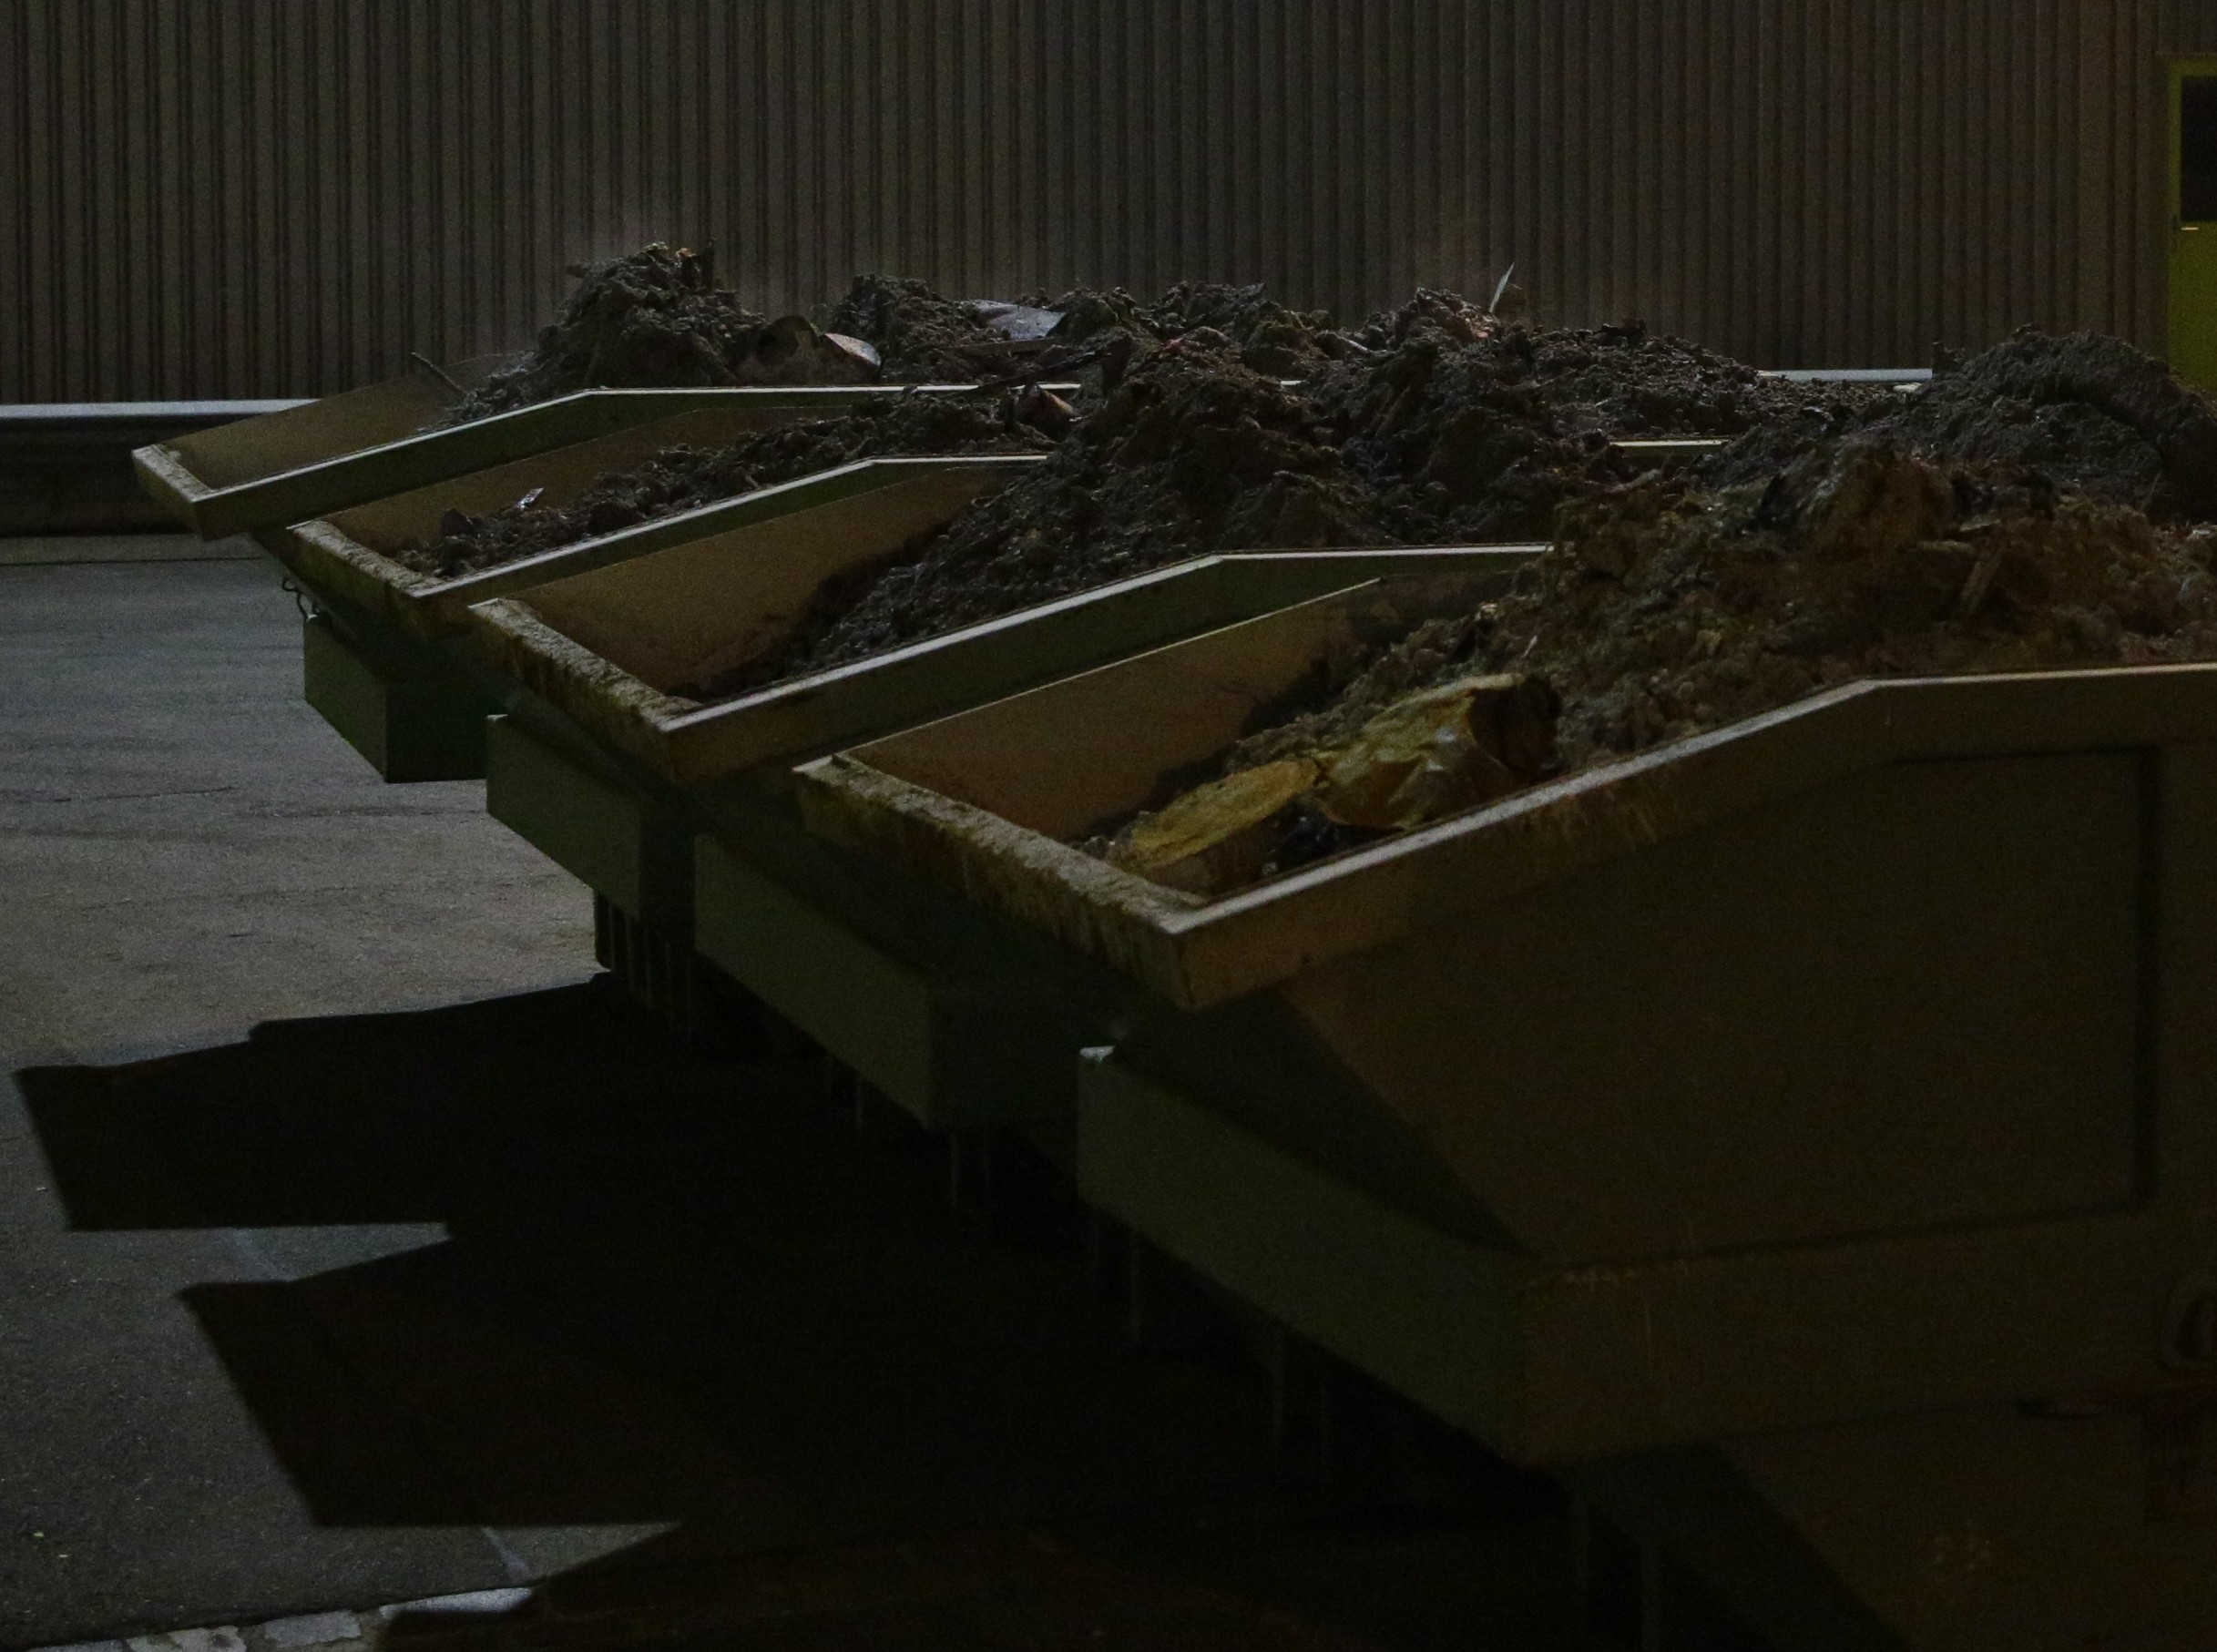
\includegraphics[width=10cm]{bilder/12_schlacke.jpg}}
\end{center}

\subsection{19:00 Uhr}
\label{sec-2-12}
Nach ungefähr zwei Stunden war die Führung dann zu Ende.  Gewisse
Teile der Führung waren etwas abstrakt. Insgesamt war es jedoch ein
sehr interessanter Besuch.  Es war erstaunlich zu sehen wie viel aus
Abfall noch gemacht wird und wie viel Aufwand betrieben wird um noch
das letzte Bisschen verwertbarer Rohstoff zu extrahieren.
Bedenklich fand ich jedoch wie die nicht verwertbaren Reste gelagert
werden. Zwar sind der Staub und die Schlacke einer KVA nicht
so schädlich wie bei einem AKW. Allerdings fragt man sich schon
ob es wirklich gut für die Nachwelt ist wenn man das Zeugs einfach
in Säcken unter dem Boden verscharrt.

\section{Funktionsweise der KVA im Überblick}
\label{sec-3}

\begin{center}
\frame{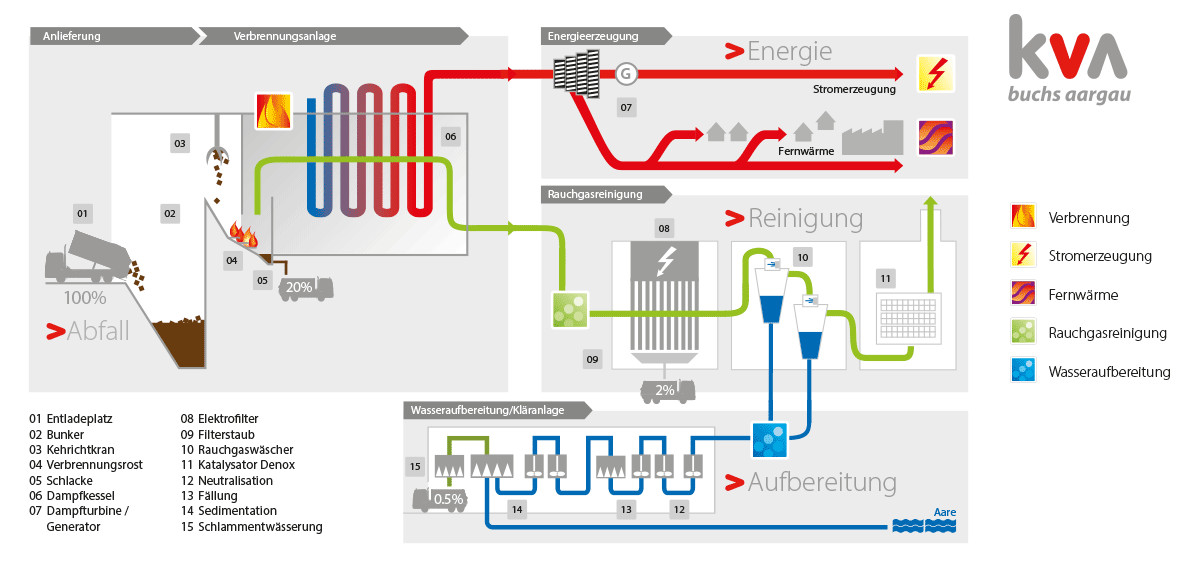
\includegraphics[width=13cm]{bilder/13_anlage.jpg}}
\end{center}

Hier nochmal die Funktionsweise der Anlage zusammengefasst.  Zuerst
wird der Lastwagen samt dem Müll gewogen um den Preis angegeben zu
können. Anschliessend entlädt der LKW seine Fracht in den Bunker.

Von dort wird er mit dem Kehrichtkran auf den Verbrennungsrost
transportiert welcher sich stetig durch den Ofen bewegt und dadurch
dem Feuer konstant neue Nahrung liefert. Bei der Verbrennung entsteht
Schlacke welche ca. 20 \% der zuvor verfeuerten Abfallmasse ausmacht.
Die Schlacke wird dann zu einer Deponie in Fricktal gebracht, wo sie
dann noch nach verwertbarem Metall durchsucht wird.

Die Hitze der Verbrennung wird genutzt um Wasser im Dampfkessel zu
erhitzen.  Der daraus entstehende Dampf treibt eine Turbine zur
Stromproduktion an. Die restliche Wärme wird zum Heizen verwendet und
an Abnehmer in der Umgebung weitergeleitet.

Die Rauchgase des Feuers werden zuerst durch einen Elektrofilter
geführt in welchem durch elektrostatische Ladung die ersten Partikel
aus dem Rauch gefiltert werden. Der dabei entstehende Staub macht etwa
2 \% des verbrannten Mülls aus.

Im nächsten Schritt wird das Rauchgas noch mit Wasser durchmischt und
so noch weiter von Schadstoffen gereinigt. Was in etwa 99 \% der
Schadstoffe entfernt. Nachdem der Rauch von einem Katalysator noch von
Stickstoffoxiden befreit wurde, wird er anschliessend in durch den
Kamin in die Umwelt gelassen.

Das Wasser welches durch den Reinigungsprozess des Rauchgases
verschmutzte wird vor der Rückführung in die Aare auch noch in einem
mehrstufigen Prozess gereinigt. Die Reste davon sind zum einen
Quecksilber, Gips sowie noch etwas unbrauchbarer Schlamm. Da das
Wasser noch stark Salz haltig ist kann es nur verdünnt wieder in die
Aare geleitet werden. Womit der Prozess dann abgeschlossen ist.